    %\documentclass[12pt,preprint]{aastex}
    \documentclass[twocolumn]{emulateapj}
    \usepackage{float,amsmath}
    \usepackage{graphicx}
    \usepackage{natbib}
    \usepackage{color}
    \usepackage{hyperref}
    \citestyle{aa}
    
    
    
    \newcommand{\vdag}{(v)^\dagger}
    \newcommand{\volt}{{v}}
    \newcommand{\vis}{{V}}
    \newcommand{\sky}{{\rm sky}}
    \newcommand{\bmvolt}{{a}}
    \newcommand{\beam}{{A}}
    \newcommand{\thhat}{{\hat\theta}}
    %\newcommand{\fngexp}{{e^{\frac{2\pi i\nu\vec{b}\cdot\thhat}{c}}}}
    %\newcommand{\ifngexp}{{e^{-\frac{2\pi i\nu\vec{b}\cdot\thhat}{c}}}}
    \newcommand{\fngexp}{{e^{2\pi i\nu\vec{b}\cdot\thhat/c}}}
    \newcommand{\ifngexp}{{e^{-2\pi i\nu\vec{b}\cdot\thhat/c}}}
    \newcommand{\dfngexp}{{e^{2\pi i\nu \Delta \tau}}}
    %\newcommand{\myemail}{skywalker@galaxy.far.far.away}
    
    \shorttitle{HERA dish reflectometry }
    \shortauthors{Patra et al.}
    
    \def\UCB{\altaffilmark{1}}
    \def\UCBtxt{\affil{\altaffilmark{1}University of California, Berkeley, nipanjana@berkeley.edu}}
    \def\ASU{\altaffilmark{2}}
    \def\ASUtxt{\affil{\altaffilmark{2}Arizona State University, School of Earth and Space Exploration, e-mail: t\_nithyanandan@asu.edu}}
    
    \def\myemail{\altaffilmark{$\dagger$}}
    \def\myemailtxt{\altaffiltext{$\dagger$}{e-mail: nipanjana@berkeley.edu}}
    \begin{document}
    
    \title{THE HYDROGEN EPOCH OF REIONIZATION ARRAY DISH III : MEASURING CHROMATICITY OF PROTOTYPE ELEMENT WITH REFLECTOMETRY. } 
    %\maketitle
    
    \author{
    Nipanjana Patra\UCB\myemail,
    Aaron~R.~Parsons\UCB,
    David~R.~DeBoer\UCB,
    Nithyanandan Thyagarajan\ASU,
    Aaron  Ewall-Wice\altaffilmark{7},
    Gilbert Hsyu\UCB, 
    Tsz Kuk Leung\UCB,
    James E. Aguirre\altaffilmark{10}, Paul  Alexander\altaffilmark{5}, Zaki S. Ali\altaffilmark{1}, Adam P. Beardsley\altaffilmark{2}, Gianni  Bernardi\altaffilmark{11, 13}, Judd D. Bowman\altaffilmark{2}, Richard F. Bradley\altaffilmark{8}, Chris L. Carilli\altaffilmark{9}, Carina  Cheng\altaffilmark{1}, Cherie~K.~Day\UCB, Eloy  de~Lera~Acedo\altaffilmark{5}, Joshua S. Dillon\altaffilmark{1}, Gcobisa  Fadana\altaffilmark{13}, Nicolas  Fagnoni\altaffilmark{5}, Randall  Fritz\altaffilmark{13}, Steve R. Furlanetto\altaffilmark{4}, Brian  Glendenning\altaffilmark{9}, Bradley  Greig\altaffilmark{12}, Jasper  Grobbelaar\altaffilmark{13}, Bryna J. Hazelton\altaffilmark{14, 15}, Jacqueline N. Hewitt\altaffilmark{7}, Daniel C. Jacobs\altaffilmark{2}, Austin  Julius\altaffilmark{13}, MacCalvin  Kariseb\altaffilmark{13}, Saul A. Kohn\altaffilmark{10}, Anna Lebedeva\UCB, Telalo  Lekalake\altaffilmark{13}, Adrian  Liu\altaffilmark{1, 16}, Anita  Loots\altaffilmark{13}, David  MacMahon\altaffilmark{1}, Lourence  Malan\altaffilmark{13}, Cresshim  Malgas\altaffilmark{13}, Matthys  Maree\altaffilmark{13}, Zachary  Martinot\altaffilmark{10}, Nathan  Mathison\altaffilmark{13}, Eunice  Matsetela\altaffilmark{13}, Andrei  Mesinger\altaffilmark{12}, Miguel F. Morales\altaffilmark{14}, Abraham R. Neben\altaffilmark{7},  Samantha  Pieterse\altaffilmark{13}, Jonathan C. Pober\altaffilmark{3}, Nima  Razavi-Ghods\altaffilmark{5}, Jon  Ringuette\altaffilmark{14}, James  Robnett\altaffilmark{9}, Kathryn  Rosie\altaffilmark{13}, Raddwine  Sell\altaffilmark{13}, Craig  Smith\altaffilmark{13}, Angelo  Syce\altaffilmark{13}, Max  Tegmark\altaffilmark{7}, Peter K.~G. Williams\altaffilmark{6}, Haoxuan  Zheng\altaffilmark{7}
    }
    
    \altaffiltext{1}{Department of Astronomy, University of California, Berkeley, CA}
    \altaffiltext{2}{School of Earth and Space Exploration, Arizona State University, Tempe, AZ}
    \altaffiltext{3}{Physics Department, Brown University, Providence, RI}
    \altaffiltext{4}{Department of Physics and Astronomy, University of California, Los Angeles, CA}
    \altaffiltext{5}{Cavendish Astrophysics, University of Cambridge, Cambridge, UK}
    \altaffiltext{6}{Harvard-Smithsonian Center for Astrophysics, Cambridge, MA}
    \altaffiltext{7}{Department of Physics, Massachusetts Institute of Technology, Cambridge, MA}
    \altaffiltext{8}{National Radio Astronomy Observatory, Charlottesville, VA}
    \altaffiltext{9}{National Radio Astronomy Observatory, Socorro, NM}
    \altaffiltext{10}{Department of Physics and Astronomy, University of Pennsylvania, Philadelphia, PA}
    \altaffiltext{11}{Department of Physics and Electronics, Rhodes University, PO Box 94, Grahamstown, 6140, South Africa}
    \altaffiltext{12}{Scuola Normale Superiore, Pisa, Italy}
    \altaffiltext{13}{SKA-SA, Cape Town, South Africa}
    \altaffiltext{14}{Department of Physics, University of Washington, Seattle, WA}
    \altaffiltext{15}{eScience Institute, University of Washington, Seattle, WA}
    \altaffiltext{16}{Hubble Fellow}
    
    \begin{abstract}
    Spectral structures from instrumental systematic effects is the current
    limiting factor for the experiments attempting to detect the redshifted 21~cm
    signal from the Epoch of Reionization (EoR). 
    Recent advances in the delay spectrum methodology for measuring the
    21~cm EoR power spectrum have brought new attention to the impact of
    an antenna's frequency \textbf{response} has on the viability of
    making this challenging measurement.
    %Systematics are specific to
    %instruments and their direct measurement or estimation is not always
    %straightforward. 
    %The Hydrogen Epoch of Reionization Array (HERA) uses the delay
    %spectrum technique for estimating of 21~cm power spectrum. 
    In particular, \textbf{this methodology} provides a somewhat straightforward relationship
    between time-domain reflectometry profiles of an instrument that can be directly
    measured with a vector network analyzer (VNA) and the power spectrum modes accessible
    to a 21~cm EoR experiment.
    %In a unique way, the
    %delay spectrum technique directly translates to reflectometry in case of
    %measuring instrumental response and allows the direct measurement of systematic
    %effects in individual array element.  
    In this paper, we derive the explicit relationship between $S_{11}$ measurements
    made by a VNA and the extent of \textbf{additional foreground contamination in delay space}.
    \textbf{In the light of this mathematical framework}, we examine
    the spectral chromaticity of a prototype antenna element which will
    constitute the Hydrogen Epoch of Reionization Array (HERA) 
    between 100 and 200~MHz.
    These reflectometry measurements exhibit \textbf{additional} structure relative
    to electromagnetic simulations, but we find 
    that even without \textbf{any further design improvement}, such an antenna element
    will support measuring $k$ modes with line-of-sight components of
    $k_{\parallel} >0.2h$ Mpc$^{-1}$.  
    %The performance is significantly better at the high frequency subbands of observation. 
    We also find that when combined with the powerful foreground weighting methods used in optimal
    quadratic estimation,
    HERA prototype elements \textbf{could successfully measure the
    power spectrum at spatial modes as low as $k_{\parallel} > 0.1h$~Mpc$^{-1}$. This study represents a major step towards 
    understanding the HERA antenna element. It also highlights an
    important method for characterizing instrument response for future
    experiments designed to detect the 21~cm EoR power spectrum using a reflector-type antenna. } 
    \end{abstract}
    
    
    \section{\textbf{Introduction}}
    
    Since it was first proposed in \cite{1997ApJ...475..429M, Shaver_et_al1999}, \textbf{measurement of redshifted} 21~cm
    emission from neutral hydrogen in our early universe has gained attention as a
    powerful probe of both cosmology and astrophysics.  While the science case for
    21~cm cosmology, particularly during the Epoch of Reionization, is well
    established (see, e.g.,
    ~\cite{furlanetto_et_al2006, morales_wyithe2010, pritchard_loeb2012}),
    the technical path toward measuring this signal has been extremely challenging.  The
    weakness of \textbf{the} hyperfine line keeps the 21~cm signal below opacity throughout
    cosmological history, but it also creates sensitivity and calibration
    challenges that are yet to be fully solved.  With noise temperatures dominated
    by sky noise and foregrounds four to five orders of magnitude
    brighter than the signal even in the coldest patches of the sky, 
    sky-averaged 21~cm monopole experiments such as
    EDGES; ~\citep{Bowman_et_al2010},
    BIGHORNS; ~\citealt{2015PhDT........65V},
    SARAS; ~\citep{Patra_et_al2015, Patra_et_al2013} ,
    SCIHI; ~\citep{2015PhDT........65V},
    HYPERION; ~\citep{presley_et_al2015}
    % XXX others?
    and 21~cm reionization power spectrum experiments such as
    the LOw Frequency ARray (LOFAR; ~\citealt{van_Haarlem_2013}),
    the Murchison Widefield Array (MWA; ~\citealt{Tingay_2013}),
    the Giant Metre-wave Radio Telescope (GMRT; ~\citealt{Paciga_et_al2011}),
    the Donald C. Backer Precision Array to Probe the Epoch of Reionization (PAPER; ~\citealt{parsons_et_al2010}),
    the Hydrogen Epoch of Reionization Array (HERA; ~\citealt{deBoer_2016}),
    and the future Square Kilometre Array (SKA; \footnote{www.skatelescope.org}~\citealt{2013ExA....36..235M})
    must furnish both their foreground suppression limits given their system performance at levels significantly
    beyond anything previously achieved in radio telescopes operating below 1 GHz.
    
    One of the most problematic effects these experiments face is the instrument
    chromaticity \textbf{that are instrument specific and have unique manifestation in the measured data}.  The spectral dimension of    
    21~cm reionization experiments is of vital
    importance; for line emission, this coordinate translates to a line-of-sight distance
    that can be used to construct three-dimensional maps (and power spectra) of emission,
    as well as probe the evolution of 21~cm emission over cosmological timescales.
    The response of a radio telescope --- either a single dish
    or an interferometer --- versus spectral frequency, modulates spectrally smooth foregrounds,
    contaminating spectral modes that might
    otherwise be used to measure reionization ~\citep{datta_et_al2010, trott_et_al2012, vedantham_et_al2012, 2012ApJ...752..137M, liu_et_al2014a}. \textbf{  Moreover, measurement sensitivity could be increased by increasing the collecting area of the element using reflector structures that  results in increased elementsize.  However, the chromaticity of
  a reflector dish scales with its diameter}, putting the
    needs of foreground suppression and signal sensitivity in direct tension with one
    another. 
    %In addition to that, systematic effects are unique to each instrument and their manifestation 
    %is different in each dataset.
    
    A major step forward for the field of 21~cm cosmology has been the development
    of a mathematical description of telescope chromaticity, how it varies with
    element separation (or telescope diameter), and what it implies for distinguishing
    foreground emission from the cosmological 21~cm signal~\textbf{\citep{Parsons_et_al_2012, vedantham_et_al2012, trott_et_al2012, 2014PhRvD..90b3018L, 2014PhRvD..90b3019L, 2015PhRvD..91b3002D,nithya_et_al2013,  Thyagarajan_et_al2015}.}  The ``wedge'', as it is
    colloquially known, describes a linear relationship between the separation between elements
    in an interferometric baseline and the maximum line-of-sight Fourier mode\footnote{Assuming
    a flat sky and using appropriate
    cosmological scalars,
    the spectral axis, $\nu$, and angle on the sky, $\vec\theta$, translate to coordinates in
    a three-dimensional volume at cosmological distances.  In describing the spatial power spectrum of
    emission in this volume $P(\vec k)$, we use the three-dimensional wave vector 
    $\vec k\equiv(k_\parallel,\vec k_\perp)$, where $k_\parallel$ is aligned with the
    spectral axis, $\nu$, and $\vec k_\perp$ lies in the plane of the sky.}
    that may be occupied by smooth spectrum foreground emission.  At low-order $k_\parallel$ modes
    within the limits of the wedge,
    foreground contamination may be suppressed through a combination of calibration and model 
    subtraction.  However, calibration or modeling errors rapidly re-establish the characteristic
    wedge pattern~\textbf{\citep{2016MNRAS.461.3135B}.  Outside of the wedge, foreground contamination drops rapidly 
    ~\citep{pober_et_al2013, 2014PhRvD..89b3002D,  Thyagarajan_et_al2015, Saul_et_al2016}}, provided that the spectral responses
    of antenna elements and analog electronics are sufficiently smooth\footnote{Here, we distinguish
    the chromaticity of the elements in isolation from the chromaticity inherent to
    element separation in an interferometric baseline.}.  In the avoidance-based
    foreground strategy employed by PAPER ~\citep{parsons_et_al2014, Ali_et_al2015}, these modes
    may be targeted as the lowest risk path for constraining 21~cm reionization in the near term.
      
    % XXX document map
    The efficacy of foreground removal from the measured data
    critically limits the 21~cm power spectrum measurements. The delay
    transformation technique of foreground removal, introduced by
    ~\citep{Parsons_Backer_2009, Parsons_et_al_2012}, computes the Fourier
    transform of the visibility measured by an interferometer and produces a
    spectrum, referred to as the delay spectrum hereafter, which is a function of
    the geometric time delay corresponding to the physical length of the baseline
    between two antennas. For the visibilities measured over a wide field across a
    wide frequency bandwidth, the delay spectrum consists of the convolution of the instrument
    response with the foreground signal, and the 21cm power spectrum, hereafter
    referred to as the EoR signal.
    %The complex visibility measured by an interferometer is a convolution of the instrument response with the true sky response in the UV plane. Therefore, when Fourier transformed, the delay spectrum is the multiplication of the sky response with the instrument response in the delay domain.
    The technique exploits the smooth spectral characteristics of the foreground
    and for a %widefield wide bandwidth
     visibility measurement by an interferometer
    with a baseline $b$, confines the foreground contribution to the computed delay
    spectrum within the largest possible time delay, $\tau_{g} = b/c$, corresponding to
    the given baseline length. \textbf{In reality, however, foregrounds show a response beyond the maximum geometric delay    
    due to broadband spectrum of the foreground sources and chromatic instrument response. For an ideal system, this 
    is a rapidly diminishing response beyond $\tau_{g}$ spanning the delay range corresponding to the inverse of the  
    measurement bandwidth. }
    Beyond this limit, for an ideal system performance, the delay spectrum would be
    dominated by any signal with spectral and spatial
    fluctuations over small scales, such as the EoR signal.  The interaction between the sky signal and instrument response can
    alter the relative contribution of the foreground, and the
    EoR signal at a given delay and influence the detectability of the EoR
    signal. Such interactions may cause the foreground to spill
    over into higher delays and push the upper limit of the foreground and
    systematics contaminated delay modes to much higher delays \textbf{contaminating the EoR window .} \\
    \begin{figure*}
    \centering
    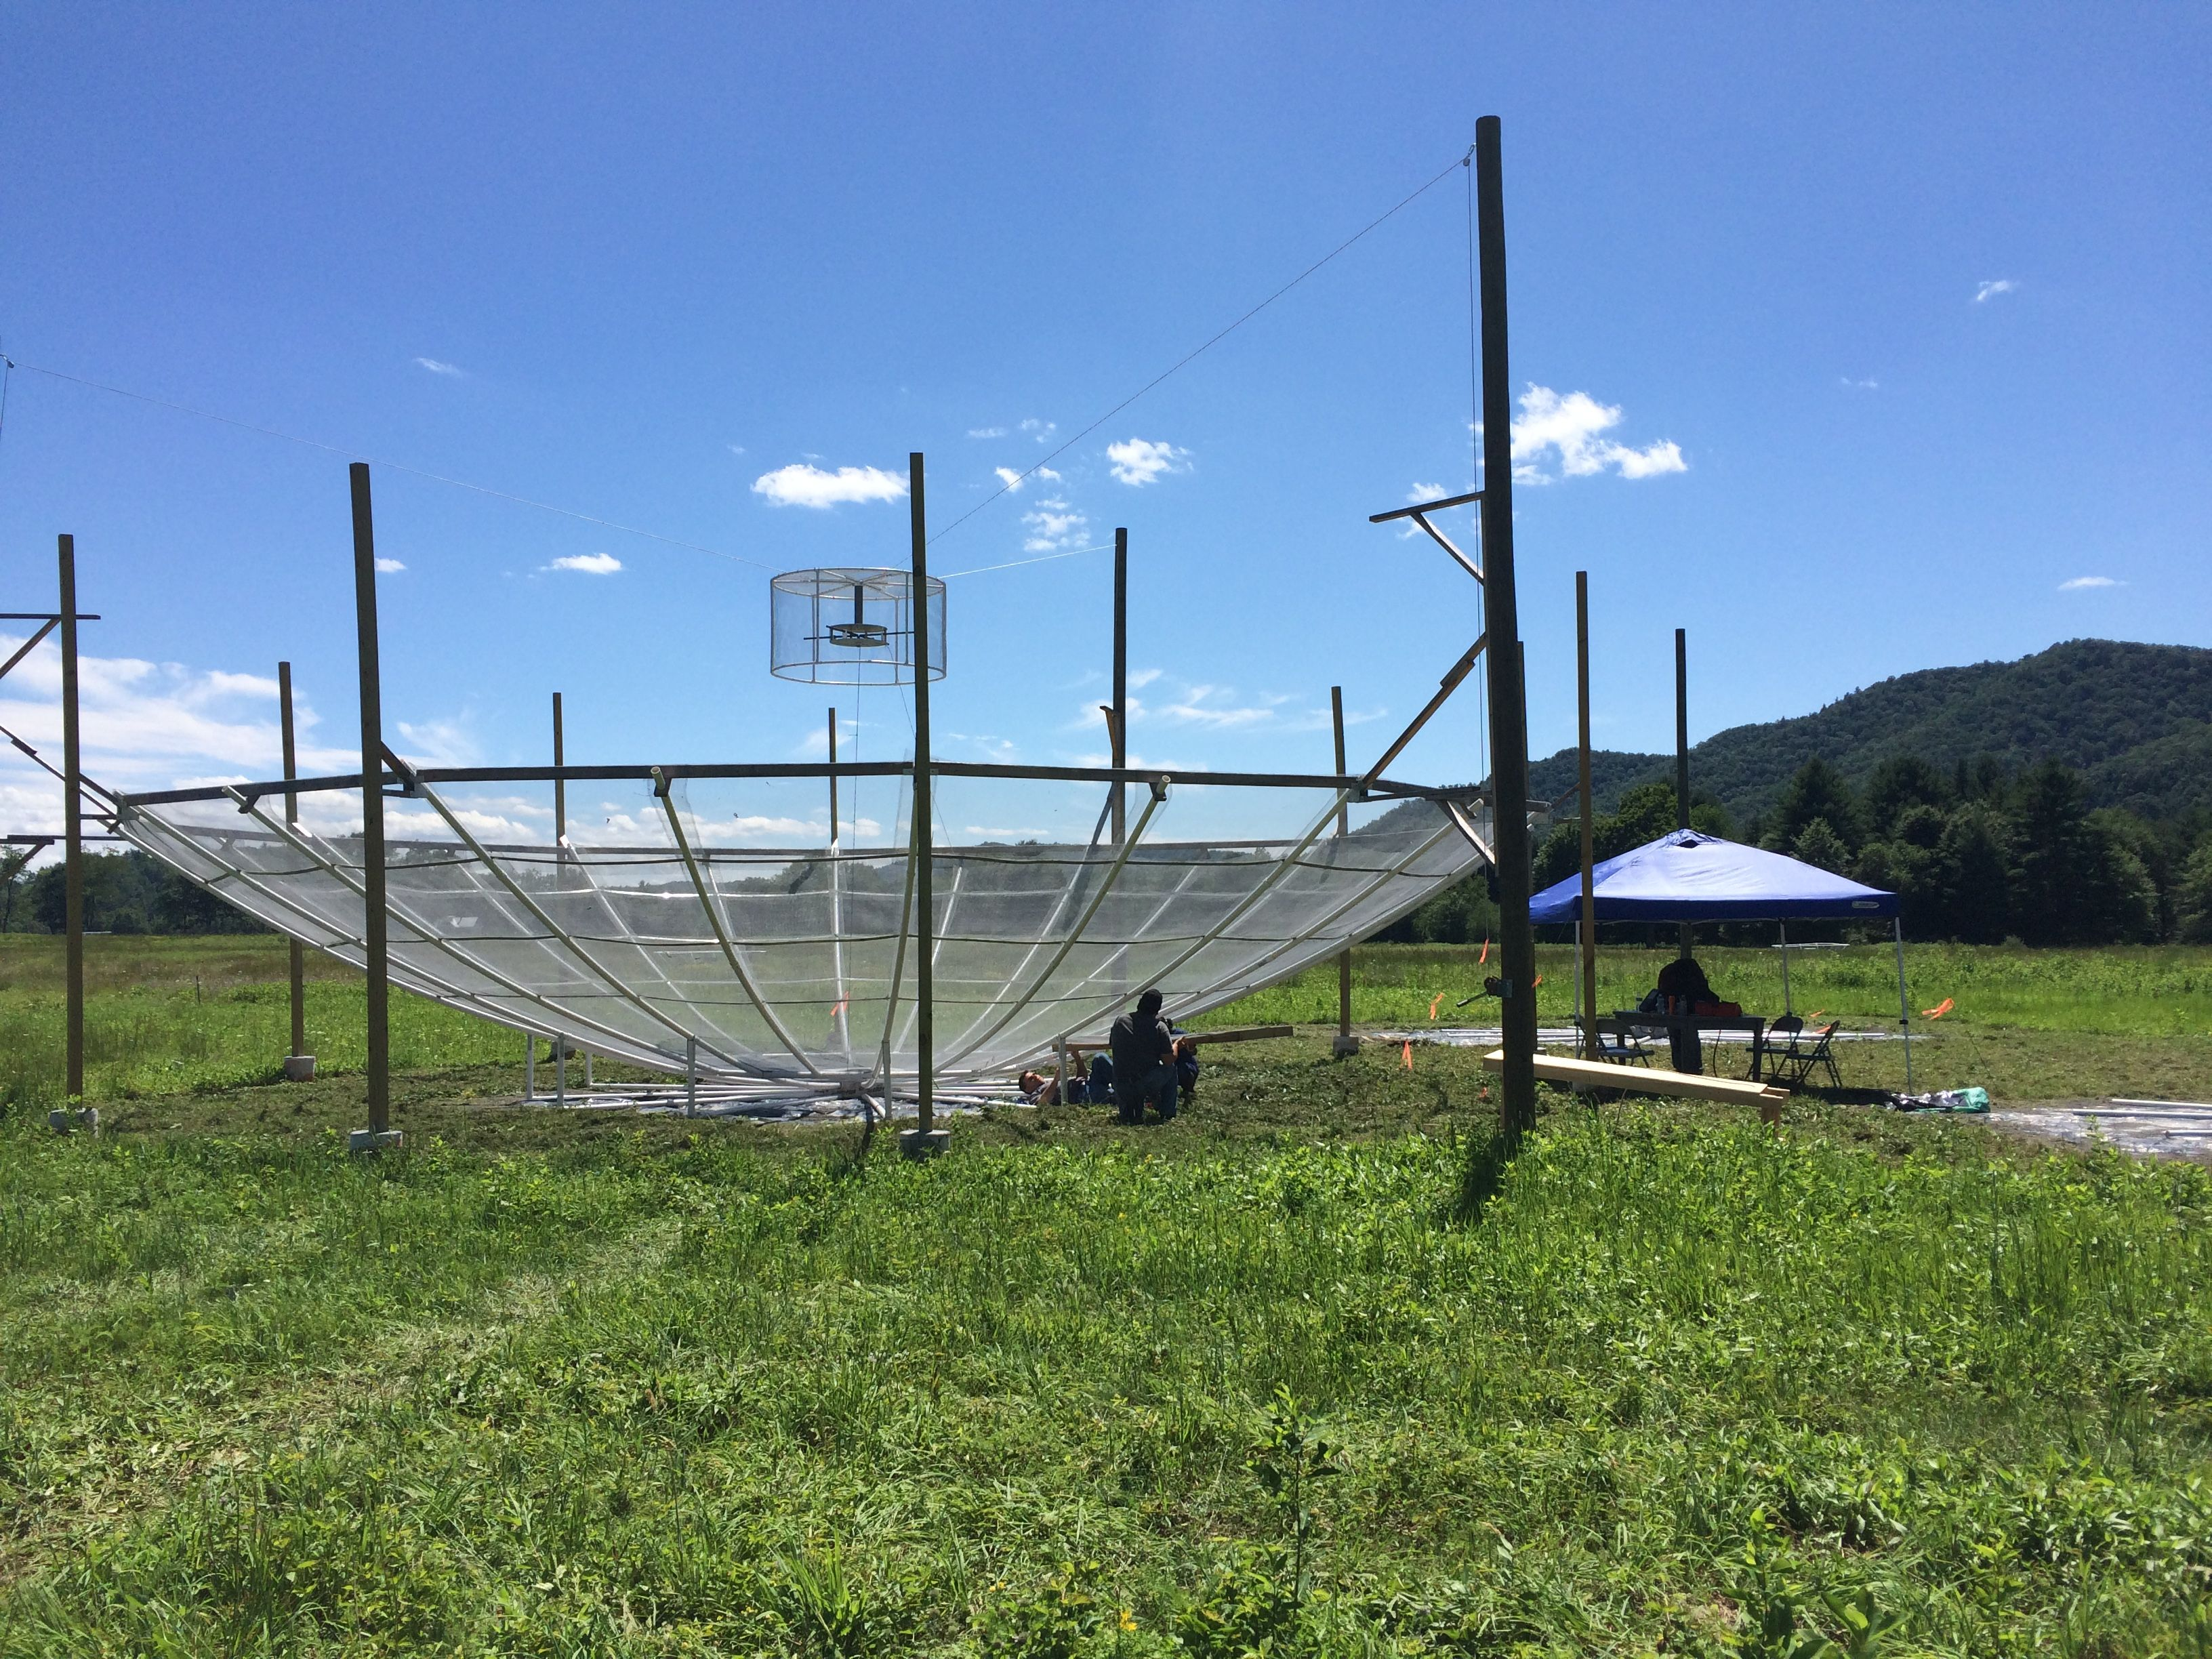
\includegraphics[trim={2cm 20cm 30cm 15cm},clip, totalheight=0.3\textheight]{plots/heradish.jpg}
    \caption{A prototype HERA element at the Green Bank NRAO site consisting of a crossed dipole feed and a parabolic reflector dish.}
    \label{fig:heradish}
    \end{figure*}
    In this paper, we use reflectometry measurements to
    investigate the delay-domain performance of 
    \textbf{a prototype 14-m parabolic reflector dish and a crossed dipole feed (figure \ref{fig:heradish}) that are proposed to be used in HERA, operating 
    from 100 to 200~MHz. For clarity, the return loss of the feed when measured off of the dish will be referred to as ``feed return loss" hereafter. The dish-feed assembly, when the feed is placed at the focal point of the dish is referred to as ``HERA element" hereafter. }
    %Reflectometry measurements are carried out across a wide bandwidth on a
    %prototype HERA element in Green Bank, WV (Figure \ref{fig:heradish}), and the
    %results are interpreted in light of the delay spectrum technique of power
    %spectrum estimation and inverse covariance weighting method of foreground
    %suppression. 
    This paper is one in a series of five papers that studies the time and frequency domain simulation of  HERA element~\citep{Ewall-Wice_et_al2016}, ~\citep{ddboer_et_al2016}, beam pattern measurements~\citep{Neben_et_al2016}, and foreground limits ~\citep{Thyagarajan_et_al2016}. We compare 
    reflectometry measurements to the simulated specification for the spectral performance of a HERA element ~\citep{ddboer_et_al2016} and to the limits of EoR to foreground power ratio established by ~\citep{Thyagarajan_et_al2016}. 
    In this paper, Section 2 briefly describes the delay spectrum for the ideal and
    non-ideal performance of a two element interferometer. Section 3 describes the
    reflectometry measurements and establishes the connection between visibility
    measurements and reflectometry. Reflectometry results are described in Section
    5. Section 6 evaluates the performance of the HERA element for detection of the
    21~cm power spectrum.
    
    
    \section{\textbf{Visibility measurements by a two element interferometer in the delay domain}}

    Consider a two element interferometer with a baseline $\vec b$. If we denote the electric field sky signal in the direction $\thhat$ \textbf{at a frequency $\nu$} by $\volt_\sky(\vec \theta, \nu)$, then the voltage output of each antenna may be written as,  
    
    \begin{equation}
    \volt_{1}(\thhat, \nu) = \bmvolt_{1}(\thhat,\nu)~\volt_\sky(\thhat,\nu)\nonumber\\
    \end{equation}
    \begin{equation}
    \volt_{2} (\thhat, \nu)= \bmvolt_{2}(\thhat,\nu)~\volt_\sky(\thhat,\nu)~\fngexp\nonumber\\
    \end{equation}
    
    \textbf{where $\bmvolt_{1}$, $\bmvolt_{2}$ are the voltage gain pattern of the two antennae.}
    Hence, the visibility measured by the interferometer may be written as, 
    \begin{equation}
    \vis(\vec b, \nu) =  \int  \volt_{1}(\thhat,\nu)~  \volt_{2}^{*} (\thhat, \nu)~ \ifngexp d\Omega
    \label{eq1}
    \end{equation}
    
    We define the antenna cross power pattern as  $\beam(\thhat,\nu)=\bmvolt_{1}(\thhat,\nu)~\bmvolt_{2}^{*}(\thhat,\nu)$ and denote the sky intensity as  $I_\sky(\thhat,\nu)=\volt_\sky(\thhat,\nu)~\volt_\sky^{*}(\thhat,\nu)$. Hence, 
    \begin{equation}
    \vis(\vec b,\nu) = \int \beam(\thhat, \nu)~ I_\sky(\thhat,\nu)~ \ifngexp d\Omega
    	%	& = & \int B(l,m, \nu) I_{sky}(l,m,\nu) exp(-2\pi i \nu \tau_{g} ) dl dm \nonumber\\
     	%	& = & B(\vec u,\nu) \ast P_{sky}(\vec u,\nu ) \nonumber\\
    	%	& = & B(\nu { |\vec b| \over c} , \nu) \ast P_{sky}(\nu { |\vec b| \over c} , \nu) \nonumber\\
    	%	& = & B(\tau_{g}, \nu) \ast P_{sky}(\tau_{g} , \nu)	
    \label{eq2}
    \end{equation}
    
    %i.e, the complex visibility is the Fourier transform of the product of the antenna beam pattern with the sky angular power spectrum. In other words, it is the convolution of the Fourier transform of the antenna power pattern with the Fourier transform of the sky. The complex visibility measured by an interferometer with a given baseline length has explicit dependence on frequency as well as implicit frequency dependence through the spatial frequency $\vec u = \nu { \vec b \over c}$ component. Since $\vec u $ is the For a given baseline length $|\vec b|$, the visibility measured at various frequencies are not only the function of frequencies but also samples different $\vec u$ in the uv space. Delay transformation technique takes the visibility measurements at different frequencies and Fourier transforms the complex visibilities. If we defineI_{sky} the Fourier conjugate of the frequency axis as $\tau$ then the equation could be written as, 
    In ~\citet{parsons_et_al2012a}, the Fourier transform of the visibility along the frequency axis was introduced,
    resulting in the delay spectrum:
    \begin{eqnarray}
    %\tilde V(\vec b, \tau) & = & \int\!\![{\beam(\vec b,\nu)*I_\sky(\vec b,\nu)] ~e^{-2\pi i\nu\tau}d\nu}%\nonumber\\	  
     \tilde V(\vec b, \tau) & = & \beam(\vec b,\tau)*I_\sky(\vec b,\tau)
                           %& = &   \left [ A(\vec b, \tau)\ast I_{sky}(\vec b, \tau) \ast \delta( \tau - \frac{{\vec {b} \cdot \thhat}}{c} )\right ] d\Omega
    \label{eq3}
    \end{eqnarray}
    % XXX rethink how to express this equation (not correct about integrated over all sky)
    % XXX define tau_g
    The convolution is carried out along the $\tau$ axis which is Fourier conjugate of the frequency $\nu$. Qualitatively, 
    delay spectrum of the visibility results from the convolution of the \textbf{instrument delay response with the delay spectrum of the sky. It is, therefore, important to determine the instrument delay response in order to determine sky delay response at a particular delay by de-convolving the delay transformed visibility by the instrument response. }
    
   The delay-transformed visibility is related to the power spectrum of redshifted
    21 cm emission by the relation, 
    \begin{equation}
     %P_{21}(k_\perp,k_\parallel) = (|\tilde V(\vec b, \tau)|^{2} \left(\frac{1}{$\Omega$\Delta B}\right)\left(\frac{D^2\Delta D}{\Delta B}\right)\left(\frac{\lambda^2}{2k_\textrm{B}}\right)^2 ,
     %\end{equation}
     %\begin{equation}
 P_{21}(k_\perp,k_\parallel) \approx |(\tilde V(\vec b, \tau)|^{2} \left(\frac{\lambda^2}{2k_\textrm{B}}\right)^2 {X^{2}Y \over \Omega \Delta B}
    \label{eq4}
    \end{equation}
    where
    \begin{equation}
      k_\perp = \frac{2\pi f}{D}\Bigg({b\over c}\Bigg), \text{ }
      k_\parallel = \frac{2\pi\tau\,f_{21}H(z)}{c(1+z)^2}, 
     \label{eq5}
    \end{equation}
   
    \begin{itemize}
    \item
     $f_{21}$:rest frame frequency of the 21~cm radiation.
     \item
    $f$: observation frequency.
    \item
    $z$: cosmological redshift corresponding to the frequency of observation.
    \item
     $\Delta B$: bandwidth centered at the observation frequency.
     \item
     $k_\textrm{B}$: Boltzmann constant.
     \item
     $D\equiv D(z)$ comoving distance along the line of sight
     \item
     $\Delta D$ the comoving distance along the line of sight corresponding to bandwidth of observation $\Delta B$.
     \item
    $H(z)= H_{0} [\Omega_\textrm{M}(1+z)^3+\Omega_\textrm{R}(1+z)^2+\Omega_\Lambda]^{1/2}$\\
     where $H(z)$ is the Hubble constant as a function of redshift, $H_{0}= 100 h$~km s$^{-1}$ Mpc$^{-1}$, $\Omega_\textrm{M}=0.27, \Omega_\textrm{R}= 0.73, \Omega_\Lambda=1-\Omega_\textrm{M}-\Omega_\textrm{R}$ are the matter, radiation and dark energy density parameters respectively.
    \item
    $X, Y$ are cosmological scalars that relates the angular dependence with spectral frequency to corresponding comoving distance.
    \end{itemize}
   % \indent In this paper, we use $$\Omega$_{M}=0.27$, $$\Omega$_{\Lambda}=0.73$, $$\Omega$_{K}=1-$\Omega$_{M}-$\Omega$_{\Lambda}$, $H_0=100 h^{-1}\,$km$\,$s$^{-1}\,$Mpc$^{-1}$, and $P(k_\perp,k_\parallel)$ is in units of K$^2 (h^{-1}$~Mpc$)^3$.
    %\indent Since both $k_{\perp}$ and $k_{\parallel}$ are functions of the delay
    %$\tau$, corresponding to the given baseline length, the redshifted 21 cm power
    %spectrum could be estimated from the delay spectrum of the visibility measured
    %by an interferometer. 
    %The sky delay spectrum from any direction $\thhat$ is
    %convolved with the delay spectrum of the instrument and would be located at the
    %delay $\tau = {\vec b \cdot \thhat \over c}$ %defined this differently earlier
     %in the delay domain. The maximum geometric delay possible for a given baseline would be $\tau_{g} ={ b \over c }$ for the direction of $\thhat = 0$, when the phase centre is halfway in between the two antennas. %The phase center is elsewhere defined as being at the center of one of the antennas.
     %Hence, the sky contribution from any direction would be confined within
    %$-\tau_{g}<\tau<\tau_{g}$. Due to the chromaticity of the sky signal as well as
    %the instrument response, the delay spectrum of the sky spills over into delays
    %with $\tau> \tau_{g}$, with a decaying amplitude [Ref to the Figure Parsons12].
    %The foreground, $P_{fg}(\tau)$, which is spectrally smooth, and the 21~cm power
    %spectrum, $P_{21}(\tau)$, which contains spectral signatures, contribute to the
    %sky delay spectrum $P_{sky}(\tau)$.Therefore, in the spill over region
   % $(\tau>\tau_{g})$, the relative strength of the smooth spectrum foreground,
    %with respect to the delay spectrum of the $I_{21}$, reduces and the 21cm delay
    %spectrum could be detectable.
    
     %In words, the sky delay spectrum from any direction $\thhat$ is convolved with the delay spectrum of the instrument and would be located at the delay $\tau = {\vec b \cdot \thhat \over c}$ in the delay domain. The maximum geometric delay possible for a given base line would be $\tau_{g} ={ b \over c }$ for the direction of $\thhat = 0$ when the phase centre is halfway in between the two antennas. Hence, the sky contribution from any direction would be confined within $-\tau_{g}<\tau<\tau_{g}$. Due to chromaticity of the sky signal as well as instrument reponse, the delay spectrum of the sky spills over the delay $\tau> \tau_{g}$ with decaying amplitude [Ref to the Figure Parsons12]. Sky delay spectrum $I_{sky}(\tau)$ is contributed by the foreground  $I_{fg}(\tau)$  which is spectrally smooth and the 21~cm power spectrum $I_{21}(\tau)$ which contains spectral signatures. Therefore, in the spill over region $(\tau>\tau_{g})$, the relative strength of the smooth spectrum foreground with respect to the delay spectrum of the $I_{21}$ reduces and the 21~cm delay spectrum could potentially be detectable. 
    
    
    %\subsection{Delay spectrum: An estimate of the 21cm power spectrum}
    %Add text here. 
     %\textbf{[ Reference to Nithya's foreground simulation work, reference to any plots on the relative contribution of the  foreground and EoR signal. ]}
    
    \section{\textbf{Effects of multiple reflections on visibility and delay spectrum}}
    
    HERA consists of \textbf{parabolic reflector antennas} which
    provide increased collecting area per array element compared to its predecessor
    experiment PAPER. Plane waves incident on a prime focus parabolic dish are focussed at the
    feed which is at the focal plane of the dish.  The mismatch between the
    impedance of free space and the feed and transmission line results in a partial
    coupling of the sky signal into the feed while the rest is reflected off the
    feed.  The reflected signal illuminates the dish and most of it is reflected
    back into the space.  However, a part of it reflects back and forth several
    times between the feed and the vertex of the dish which is shadowed by the
    feed.  Such reflections generate multiple copies of the incident sky signal of
    reduced strength at various delays and phases producing additional
    correlations in the visibilities data.  \textbf{Identical
    visibilities can result from reflections internal to the system,
    for example between antenna output and backend receiver input causing similar signal contamination in delay space. Therefore, it is necessary to measure and develop the
    understanding of the instrument delay spectrum.}  In this section we compute the visibility
    of a two element interferometer accounting for the additional reflections of
    the sky signal in between the feed and the dish vertex and the corresponding
    effects on the delay spectrum in detail. We assume two antennas with identical
    geometry and electrical parameters i.e,
    $\bmvolt_{1}(\thhat,\nu)=\bmvolt_{2}(\thhat,\nu) = \bmvolt(\thhat,\nu)$. 
    
     \subsection{Antenna Reception With Multiple Reflections}
    \label{sec:multiple}
    
    To examine the performance of an antenna and feed in the presence of multiple
    reflections, we can think of the system as a screen at a distance $F$ from a
    feed (see figure \ref{fig:sys}).  The screen reflects a factor, $\Gamma_d$, of the voltage
    and transmits $(1+\Gamma_d)$ where $\Gamma_{d}$ is the voltage reflection coefficient of dish (see, {\em e.g.} Pozar).  Similarly, the feed
    reflects $\Gamma_f$ and transmits $(1+\Gamma_f)$ where $\Gamma_{f}$ is the voltage reflection coefficient of the feed.  Both $\Gamma_{d}$ and $\Gamma_{f}$ are complex numbers that  
    are functions of frequencies. Therefore, for a given incidence of the sky voltage
    $\volt_{sky}$,  $(1+\Gamma_{d})(1+\Gamma_{f})$
    is coupled into the cable leading to the receiver backend from the feed.  Additionally, the 
    voltage that is reflected off the feed ($\Gamma_f$), is subsequently reflected off the dish by a factor
    ($\Gamma_d$) and $(1+\Gamma_{f})$ of it reenters the feed with a
    roundtrip time delay $\Delta \tau=2F/c$. Hence, if $v_{sky}$ is reflected $n$
    times in between the feed and the dish, the net voltage entering the feed after
    the $n^{th}$ reflection may be written as:
    \begin{eqnarray}
    \volt_{rec} & = &  (1+\Gamma_d) (1+\Gamma_{f}) \volt_{sky}[1+ \Gamma_{f}\Gamma_{d} \dfngexp \nonumber \\
    	&& + (\Gamma_{f}\Gamma_{d})^2  (\dfngexp)^{2}+ \nonumber \\
    &&  ....+ (\Gamma_{f}\Gamma_{d})^{n} (\dfngexp)^{n}]
    \label{eq6}
    \end{eqnarray}
    
    %\begin{figure*}[ht]
    %\begin{minipage}[b]{0.5\linewidth}
    %\centering
    %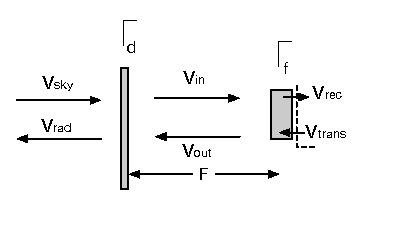
\includegraphics[width=\linewidth]{plots/microsys.pdf}
 %   \caption{Schematic diagram of signal propagation  }
    %\end{minipage}
    %\hspace{0.1cm}
    %\begin{minipage}[b]{0.5\linewidth}
    %\centering
    %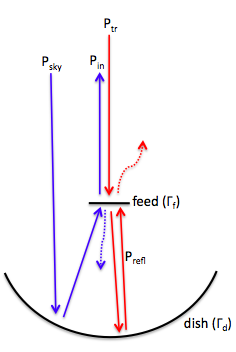
\includegraphics[width=\linewidth]{plots/reflection_cartoon.png}
    %\caption{Schematic diagram of signal propagation  }
    %\end{minipage}
    %\label{fig:sys}
    %\end{figure*}
    \begin{figure}[ht]
    \centering
    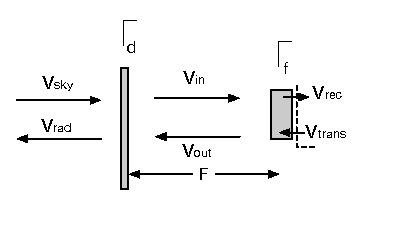
\includegraphics[width=\linewidth]{plots/microsys.pdf}
    \caption{Schematic diagram of signal propagation through the dish and the feed of during both transmission and reception. $V_{sky}$, $V_{in}$ and $V_{rec}$ represents the sky voltage, total reflected voltage from the dish that is incident on the feed and the net received voltage at the receiver input. In transmission mode, $V_{trans}$, $V_{out}$ and $V_{rad}$ are the voltage transmitted by the network analyser, the voltage output of the feed and the the net radiated voltage after reflection on the dish. $\Gamma_{d}$,  $\Gamma_{f}$ are the voltage return loss of the dish and the feed. }
    \label{fig:sys}
    \end{figure}
    
    \noindent
    %Defining $a=\volt_{rec}/\volt_{sky}$ and we see that 
    Hence,
     \begin{eqnarray}
    {\volt_{rec}\over \volt_{sky} } & = &   (1+\Gamma_d)(1+\Gamma_{f}) \displaystyle\sum\limits_{n=0}^{N} [\Gamma_{f}\Gamma_{d}\dfngexp]^{n}\nonumber\\
    & = & \frac{ (1+\Gamma_d)(1+\Gamma_{f})}{1-\Gamma_{f}\Gamma_{d}\dfngexp} 
    \label{eq7}
    \end{eqnarray}
    Note that $n=0$ is when the initial wave enters the cable at the feed (where we assume we have set our reference plane).  We identify $(1+\Gamma_d)$ as the voltage reception pattern of the antenna, denoted $\bmvolt(\thhat,\nu)$, which is a function of angle on the sky.  Additionally, $(1+\Gamma_f$) is the voltage efficiency for the feed (not a function of angle).
    
    %As an aside, note that the sum in Eq. \ref{eq:Sigma} may be evaluated we may rewrite
    %\begin{equation}
    %{\volt_{rec}\over \volt_{sky} } =  (1+\Gamma_d)(1+\Gamma_{f})\frac{1+\Gamma_{f}^{N+1}\Gamma_{d}^{N+1}(\dfngexp)^{N+1}}{1+\Gamma_{f}%\Gamma_{d}\dfngexp} \nonumber
    %\end{equation}
    %which, in the limit becomes:
    %\begin{equation}
    %{\volt_{rec}\over \volt_{sky} } = \frac{ (1+\Gamma_d)(1+\Gamma_{f})}{1+\Gamma_{f}\Gamma_{d}\dfngexp} \nonumber
    %\end{equation} 
    %since $|\Gamma_d|$ and $|\Gamma_f|$ are less than one.
    
    An accurate measurement of this quantity requires receiving $v_{sky}$ from a
    well calibrated, wideband source in the sky in the far field of the HERA
    antenna element with significant isotropic emission. \textbf{While this condition is
    hard to achieve in practice, reciprocity of the antenna performance
    in the transmission and reception mode implies the right hand side of equation
    \ref{eq7} could be measured using the return loss measurement technique with a
    vector network analyzer (VNA).} \\
    \section{\textbf{Reflectometry}} 
    Reflectometry is a method of determining the multiple reflection of any signal within 
    a system in either time or frequency domain. If applied to a radio telescope such as
     a parabolic dish, this can determine the extent to which 
    sky signal is reflected back and forth between the reflector and the feed ~\citep{2015arXiv150205862P}.
    Frequency domain reflectometry measurements are carried out on a prototype HERA in
    Green Bank, WV (figure \ref{fig:heradish}) in order to measure the instrument
    response of the feed and dish assembly and characterise the performance.  \textbf{The prototype HERA
    element} consists of a $14.5~m$ diameter parabolic reflector and a
    crossed-dipole pair as a feed. The cross dipole antenna pair is identical to
    the feed of the PAPER antenna and suspended at the focal plane of the dish
    with the support of three vertical poles. HERA elements \textbf{will be} closely spaced with
    centre to centre distance between two dishes slightly larger than the dish diameter.
    Therefore, to reduce the coupling between the adjacent dishes, the crossed
    dipole feed along with the back plane is encased in a cylindrical cage. The
    feed is raised and lowered by a pulley system mounted on the three poles.
    The focal height of the dish is 5~m.  The detail geometry and electromagnetic
    design of of the feed is presented in \cite{ddboer_et_al2016}. \\
    
    %A vector network analyser is connected via a 50feet long cable at the feed output of the HERA element and the return loss $(s_{11})$ of the HERA element is measured as a function of frequencies while the feed is suspended at the focal plane of the dish. 
    
     A VNA is connected to the HERA element via a $\approx 15$~m cable. It then transmits
    a broadband noise voltage, $\volt_{trans}$, and a factor $(1+\Gamma_f)$ of this
    voltage is radiated by the feed while the fraction $\Gamma_{f}$ returns to the
    VNA. Although the radiated signal illuminates the dish and most of it is
    radiated into free space, a fraction $\Gamma_d$ of this signal is reflected
    back towards the feed, and $(1+\Gamma_f)$ is received by the VNA.  The received
    voltage, after $n$ reflections between the dish and the feed (where again $n=0$
    is the first reflected signal at the reference plane), is therefore:
    \begin{eqnarray}
    \volt_{rec} & = &  \Gamma_f \volt_{trans} \nonumber \\
             && + \volt_{trans} (1+\Gamma_f)^2 \Gamma_{d} \dfngexp \nonumber \\
             && + \volt_{trans} (1+\Gamma_f)^2 \Gamma_{d} \dfngexp \Gamma_d\Gamma_f\dfngexp \nonumber \\
             && + \volt_{trans} (1+\Gamma_f)^2 \Gamma_{d} \dfngexp (\Gamma_d\Gamma_f\dfngexp)^2 \nonumber \\
    &&  ....+ \volt_{trans} (1+\Gamma_f)^2 \Gamma_{d} \dfngexp (\Gamma_d\Gamma_f\dfngexp)^n \nonumber \\
    \label{eq8}
    \end{eqnarray}
    Therefore, 
    \begin{equation}
    {\volt_{rec}\over \volt_{trans} } = \Gamma_f + \frac{(1+\Gamma_f)^2}{\Gamma_{f}} \displaystyle\sum\limits_{n=1}^{N} [\Gamma_{f}\Gamma_{d}\dfngexp]^{n}
    \label{eq9}
    \end{equation}
    The VNA measures the quantity $\volt_{rec}/\volt_{trans}=s_{11}$ which is the voltage reflection coefficient of the HERA element.
    The fundamental differences between the right hand side of equations \ref{eq7} and \ref{eq9} are the $n=0$ term and the multiplicative factor in front of the convergent series $\displaystyle\sum\limits_{n=1}^{N} [\Gamma_{f}\Gamma_{d}\dfngexp]^{n}$ that represents the contribution of the delayed voltage components at the VNA input, arising due to multiple signal reflections between the feed and the dish. Finally, writing $\volt_{rec}/\volt_{trans}=s_{11}$, equation \ref{eq9} can be written as,
    \begin{equation}
    s_{11} +\frac{(1+\Gamma_f)^2}{\Gamma_f}-\Gamma_f = \frac{(1+\Gamma_f)^2}{\Gamma_{f}} \displaystyle\sum\limits_{n=0}^{N} [\Gamma_{f}\Gamma_{d}\dfngexp]^{n}
    \label{eq10}
    \end{equation}
    Comparing to Eq. \ref{eq7} we find that
    \begin{eqnarray}
    {\volt_{rec}\over \volt_{sky} } & = & (1+\Gamma_d)\left[(1+\Gamma_f) + \frac{\Gamma_f}{(1+\Gamma_f)}\left(s_{11} - \Gamma_f\right)\right] \nonumber\\
     & = & \bmvolt(\thhat,\nu) \left[(1+\Gamma_f) + \frac{\Gamma_f}{(1+\Gamma_f)}\left(s_{11} - \Gamma_f\right)\right]
    \label{eq11}
    \end{eqnarray}
    When the feed return loss is measured separately, all the higher order terms of equation \ref{eq9} do not exist. In this case, $\Gamma_f = s_{11}^{f}$. Using this measurement and the VNA measurement of $s_{11}$, the quantity $v_{rec}\over v_{sky}$ is estimated. \\
    %
    \indent From this, for a two element interferometer with identical antenna elements, the ratio of the received sky intensity to true sky intensity will be, 
    \begin{eqnarray}
    {I_{rec}\over I_{sky} } & = & \Bigg|{\volt_{rec}\over \volt_{sky} }\Bigg|^2 =  \beam(\thhat,\nu)\times \nonumber\\
                 && [ |1+\Gamma_f|^2 +  2\operatorname{Re}\left(\frac{\Gamma_f}{(1+\Gamma_f)}(s_{11} - \Gamma_f)\right)  \nonumber\\ 
                 &&  + \frac{|\Gamma_f|^2}{|1+\Gamma_{f}|^2}|s_{11} - \Gamma_f|^2]    \nonumber\\
    \label{eq12}             
    \end{eqnarray}
    
    In terms of visibility, the same could be written as,  
    \begin{eqnarray}
    \vis^{mul}(\vec b,\nu) & = & \int \beam(\thhat,\nu)\times \nonumber\\
                 && \left[|1+\Gamma_f|^2 +  2\operatorname{Re}\left(\frac{\Gamma_f}{(1+\Gamma_f)}(s_{11} - \Gamma_f)\right)\right] + \nonumber\\ 
                 &&  \left[ \frac{|\Gamma_f|^2}{|1+\Gamma_{f}|^2}|s_{11} - \Gamma_f|^2  \right]  I_{sky} \ifngexp d\Omega
    \label{eq13}
    \end{eqnarray}
    Comparing equations \ref{eq13} and \ref{eq2}, the cross power generated by
    $v_{1}$ and $v_{2}$ has a spurious visibility response due to the mutual
    correlation between multiply reflected voltages represented by the second and
    the third term of the right hand side of equation \ref{eq13}. In the ideal
    case, $\Gamma_{f}=0$, in which case equation \ref{eq13} results in equation
    \ref{eq2}. The Fourier transform of this visibility spectrum along the
    frequency axis results in the delay spectrum.  In the delay domain,
    visibilities contributed to by any two voltage components from two antennas
    with no mutual delay will be located at the delay $\tau = 0$ whereas any two
    voltage components from two antennas having a mutual delay of $n\Delta \tau$
    will be centred at $n\Delta \tau$. These will result in leakage of the foreground 
    to delays where EoR power spectrum could be measured.
   % spectrum, which ultimately interferes with the 21cm power spectrum detection.
     \begin{figure*}
    \centering
    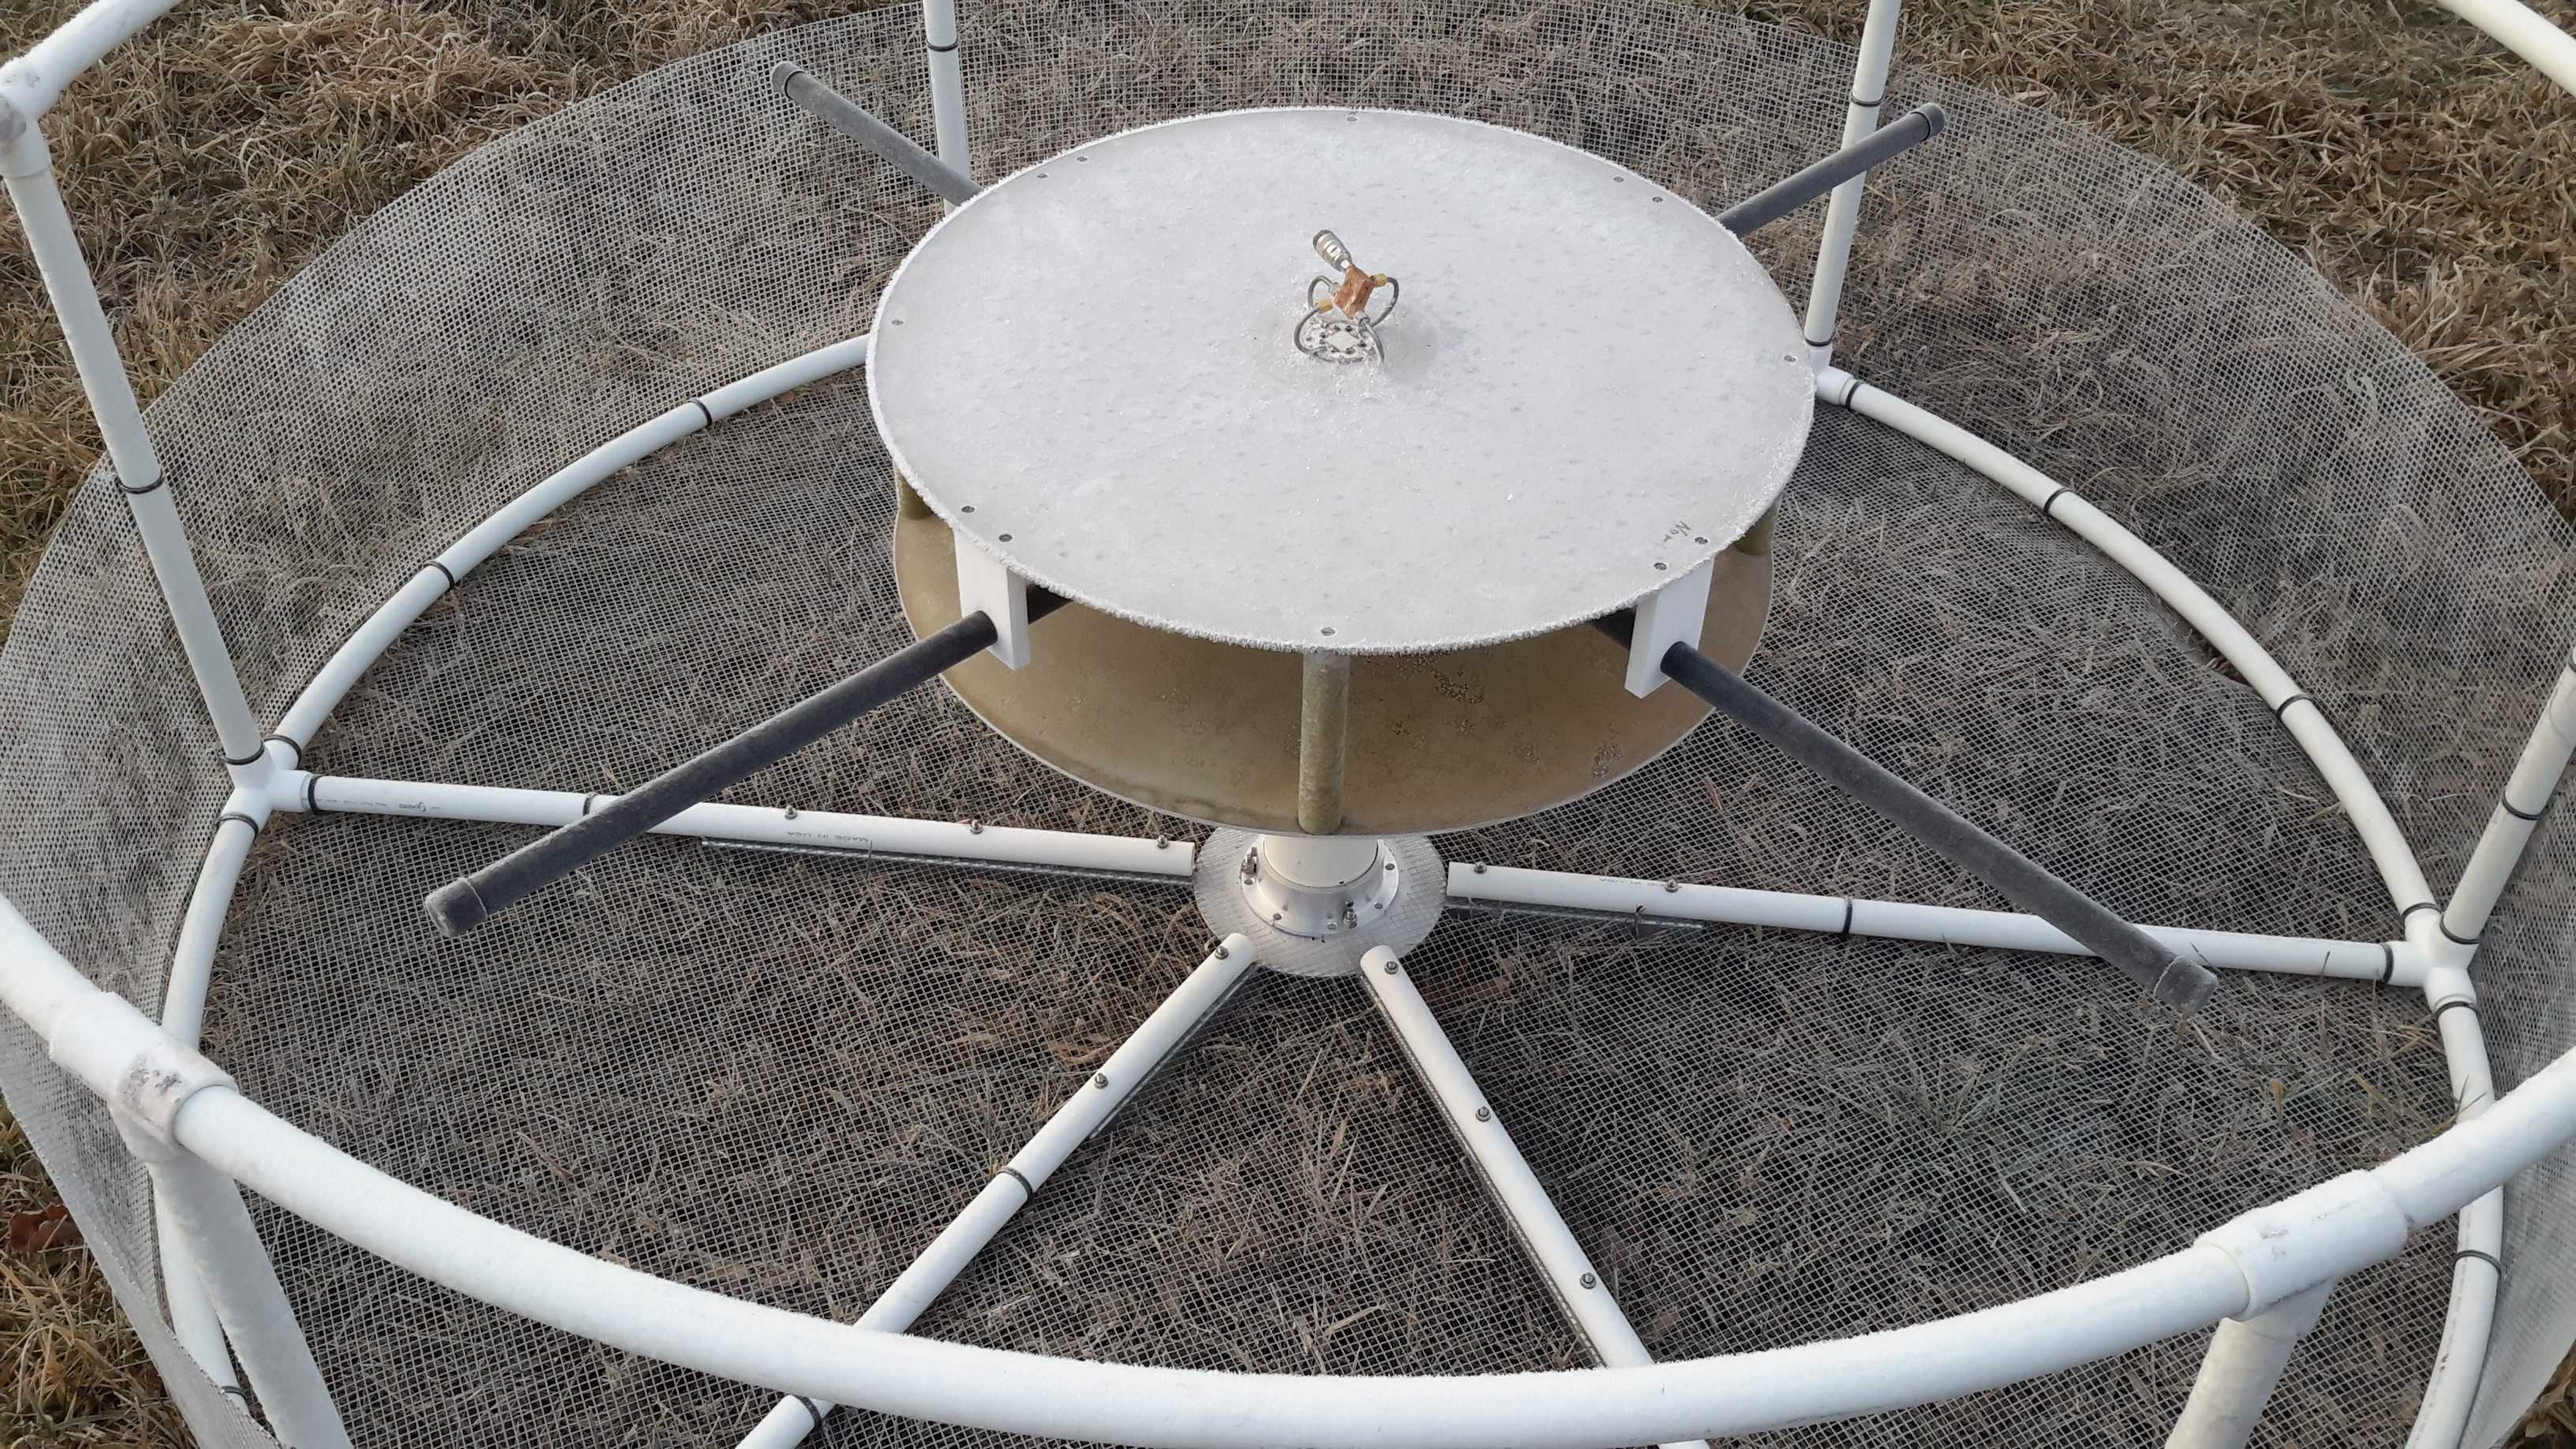
\includegraphics[trim={2cm 10cm 20cm 5cm},clip, totalheight=0.3\textheight]{plots/herafeed.jpg}
    \vspace{1.0 em}
    \caption{The HERA feed consists of a pair of crossed-dipoles over 1.72 m diameter backplane made of wire mesh. The backplane is surrounded by 0.36 m wide wire mesh around the edge resulting in encasing the crossed-dipoles in a cylindrical cage.}
    \label{fig:herafeed}
    \end{figure*}
     \section{\textbf{Results}}
    %Return loss measurements yields the instrument pass band response that would manifest in autocorrelation data of a single HERA element. Upon our assumption that two adjacent antenna elements have identical design parameters and electrical properties, this power is also a measure of the cross power or the visibility $\vis (\vec b, \nu)$ between the two antennas with a normalisation factor of $2$. 
    Return loss measurements of the feed as well as HERA element is shown in figure \ref{RL_mag_dish}. Estimated        
    delay spectra are shown in figure \ref{ds_feed_on_dish_trans}. A number of systematic effects as well as
    mathematical artifacts that are critical to this measurement and their effects
    on the corresponding estimation of the delay spectrum are discussed next. 
    
    
    
    \begin{figure*}[ht]
    \begin{minipage}[b]{0.5\linewidth}
    \centering
    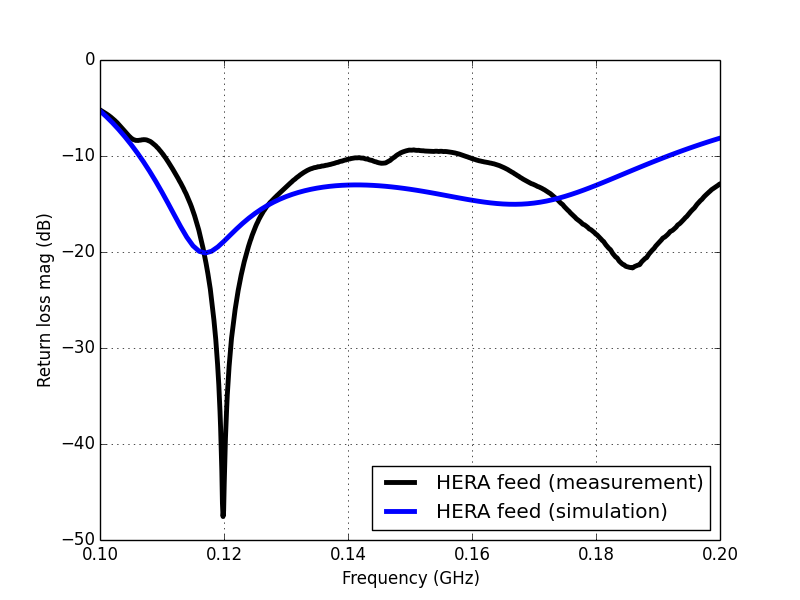
\includegraphics[angle=0, width=\linewidth]{GB_reflectometry_part3/plot/RL_feed_mag.png}
    \end{minipage}
    \hspace{0.1cm}
    \begin{minipage}[b]{0.5\linewidth}
    \centering
    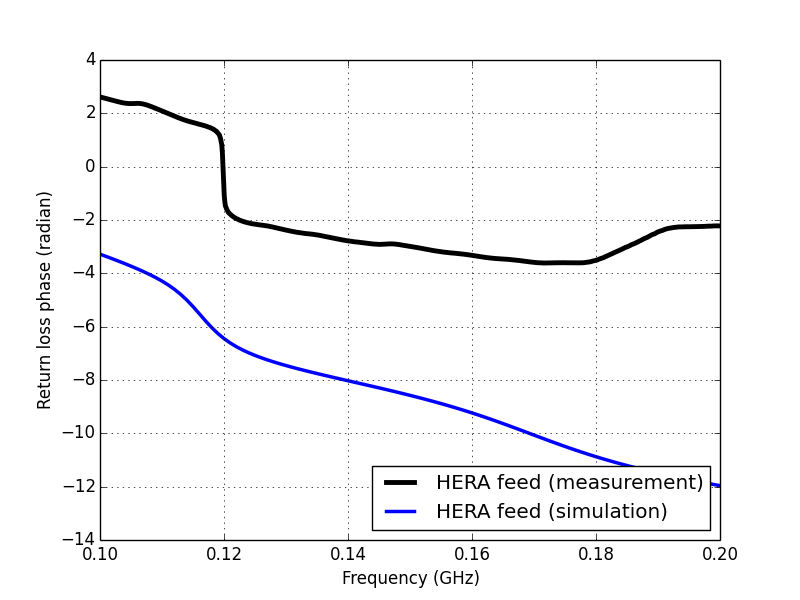
\includegraphics[angle=0, width=\linewidth]{GB_reflectometry_part3/plot/RL_feed_ph.png}
    \end{minipage}
    \vspace{0.1cm}  
    \begin{minipage}[b]{0.5\linewidth}
    \centering
    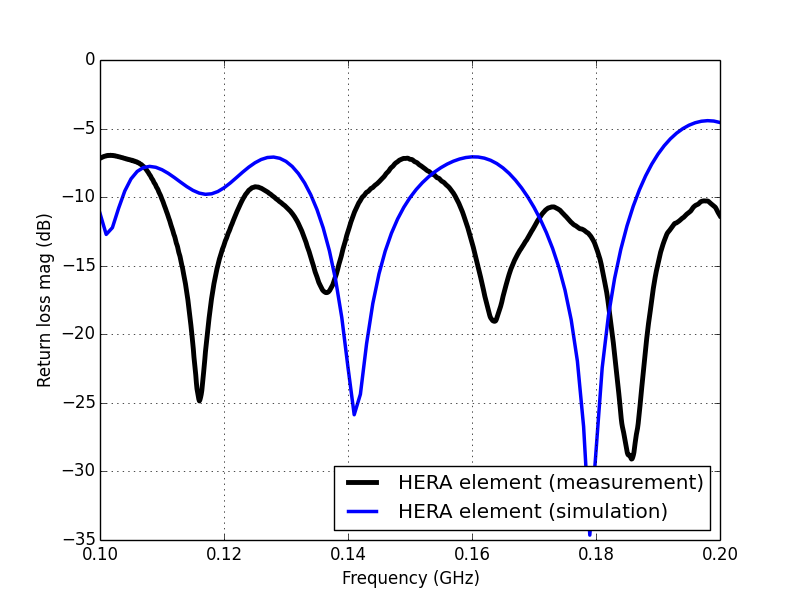
\includegraphics[angle=0, width=\linewidth]{GB_reflectometry_part3/plot/RL_HERA_mag.png}
    \end{minipage}
    \hspace{0.1cm}
    \begin{minipage}[b]{0.5\linewidth}
    \centering
    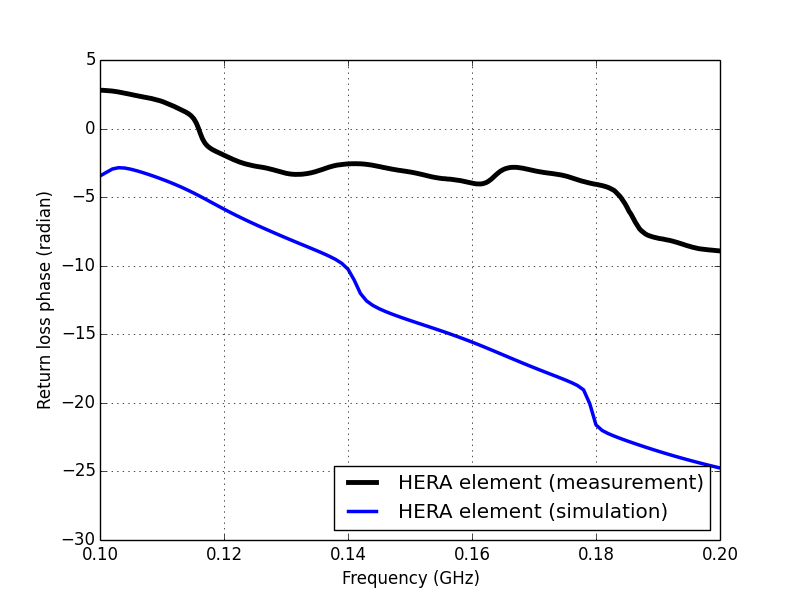
\includegraphics[angle=0, width=\linewidth]{GB_reflectometry_part3/plot/RL_HERA_ph.png}
    \end{minipage}
    \caption{Upper panel: Magnitude and phase of the return loss of the feed as simulated and measured. Both measurement and simulation shows similar level of return loss across the band with marginally better return loss at the high frequency end of the band. Lower panel: Magnitude and phase of return loss when the feed is suspended at the focal point of the dish which 5~m above the dish vertex.}   
    \label{RL_mag_dish}
    \end{figure*}
    
    \begin{figure}       
    \centering
    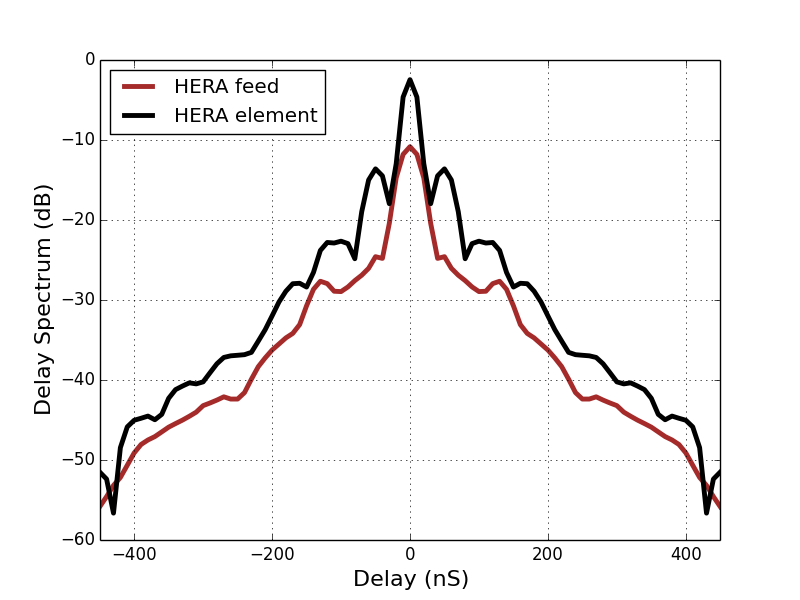
\includegraphics[width=\linewidth]{GB_reflectometry_part3/plot/ds_feed_dish.png}
    \caption{Delay spectrum of the HERA feed (brown) estimated by taking the Fourier transform of the measured return loss of power at the feed output (upper panel in figure \ref{RL_mag_dish}). The feed, when suspended on the dish results in a more complex return loss as shown in the lower panel of figure \ref{RL_mag_dish} and corresponding delay response is shown here in black. A balun with impedance transformation ratio $4:1$ is used for converting the antenna balanced output to unbalanced output voltage. Balun response is embedded in the measurements. }
    \label{ds_feed_on_dish_trans}
    \end{figure}
    
       %To estimate the delay spectrum of the dish-feed assembly i.e one single HERA element, this measurement is first corrected to map the response of the antenna from transmitting mode to receiving mode via equation \ref{zero_delay_correction}. The corrected measurement is then Fourier transformed to obtain the delay spectrum of the instrument in the receiving mode as given in equation \ref{corrected_response}. 
    %Measurement bandwidth is kept much larger than the bandwidth of operation to
    %achieve higher delay resolution. 

    
    \subsection{Zero delay response}
    %At first, the frequency domain measurement of s11 is Fourier-transformed to compute the response of the system in the delay domain. 
    
    %\subsection{\textbf{Antenna beam pattern and feed return loss}}
    %The return loss $\Gamma_{f}$ determines the amount of power coupled to the system via the feed antenna. Additionally, with each reflections, the power coupled to the system reduces by a factor of $\Gamma_{f}^{2}$. Since reflected signal results in system response in higher delay, multiple reflections of the signal off the feed and the dish would result in an exponential envelope in the delay spectrum.  The return loss of power results from the antenna impedance mismatch with the free space as well as the transmission line. While antenna beam pattern $A_{f}$ is a smooth function of frequency and should have its imprint confined to lower delays, the return loss $\Gamma_{f}$ broadens the delay spectrum. However, a smaller return loss will result in vertical shift of the delay spectrum at lower values and therefore can make the higher order reflections insignificant. 
    
    During observation, each HERA element is connected to an active balun similar
    to the ones used in the PAPER antenna which provides greater than 10dB return
    loss of power at the feed output. These baluns are currently under further design 
    improvements aiming at 10 to 20dB
    better impedance match between the feed and the backend. \textbf{The measurement presented here is done using a vector network analyzer}. \textbf{The active balun is replaced by a passive one with 4:1 impedance transformation ratio for achieving a better match to the 50~$\Omega$ transmission line}. These measurements, therefore, provide a conservative estimate for $\Gamma_{f}$ and $S_{11}$.
     %These measurements are conservative
    %estimate  for both $\Gamma_{f}$ and $s_{11}$}.
    
     While measuring the return loss
    of the dish-feed assembly, the signal transmitted by the VNA is reflected first
    from the feed. This is represented by $\Gamma_{f}$ in equation \ref{eq9}. This
    essentially represents a mismatch in between the feed and the 50~$\Omega$
    transmission line. In delay domain, this appears at the zero delay bin. The
    zero delay response is identical whether or not the feed is suspended on the
    dish. Therefore, we measure this response by measuring the feed return loss
    alone while the feed is kept on the ground facing the sky. This results in feed
    return loss alone including the surrounding cage structure but excluding the
    dish response. While $\Gamma_{f}$ fraction of incident voltage is reflected off
    the feed, $1+\Gamma_{f}$ fraction of the voltage is transmitted. In receiving
    mode, upon initial incidence, $\Gamma_{f}$ fraction of voltage is reflected
    back in to the space while $1+\Gamma_{f}$ voltage enters the feed. In receiving
    mode, in delay domain, this appears at the zero delay bin.  The using the
    return loss measurement of the feed $(\Gamma_{f})$, the return loss measurement
    $s_{11}$ of the dish and feed assembly is corrected via equation \ref{eq11} and
    the quantity of interest ${I_{rec}\over I_{sky}}$ is estimated. Figure \ref{ds_feed_on_dish_trans}
    shows the delay response of the feed alone computed from the return loss measurement of the feed alone in 
    transmission mode(brown). \textbf{Using this return loss measurement of the feed, we compute the quantity $v_{rec}/v_{sky}$. 
    and the corresponding delay spectrum is shown in black. }
    
    
    \subsection{Dish reflections}
    
    Measurement equations show the effects of multiple reflections of the sky
    signal between the feed and the dish. Any other reflections off the feed
    structure and/or any other part of the dish-feed assembly would appear at
    \textbf{delays corresponding to particular length scale. The estimated delay spectrum of the instrument is
    collectively contributed by all the reflections. The delay response of
    feed alone provides the lowest limit of
    the delay spectrum of the instrument when there is no multiple
    reflections in between the feed and the dish.  From figure
    \ref{ds_feed_on_dish_trans}, at lower delays, the reflections are dominated by
    the feed structure. Therefore, the delay spectrum in both the cases follow each
    other. Since the distance between the feed and the dish is 5 m, the roundtrip
    delay between the dish and the feed is about 30~ns. Hence, the dish
    reflections are expected to manifest themselves at an integral multiple of
    30~ns. The diameter of the feed cavity is 172~cm  which results in signal
    reflections every integral multiple of $\approx$2.86~ns. The combined effect of
    the feed and the dish dominates the delay spectrum up to $\> $50~ns after which the
    dish reflections begin to dominate and the two delay spectra deviates. }
    %With some manipulation of the equation \ref{eq10}, we can estimate
    %the dish return loss $\Gamma_{d}$ and corresponding delay spectrum as shown in
    %figure \ref{dish_delay_spectrum}.
    
    \subsection{Multiple reflection between the feed and the backend.}
    
    Another effect that \textbf{allows smooth foreground power to spill into higher delays}
    are the multiple reflection of the received signal between the feed output and
    the input of the analog backend and correlators. In our measurements, the feed
    output is connected to the VNA via a 15~m long LMR 400 cable. This length
    corresponds to a delay of $\approx$ 120~ns for the signals traveling through
    the cable. The delay spectra of both feed and feed-dish assembly shows an
    enhanced feature around this delay indicating a reflection from the VNA input.
    
     We
    measure the VNA input reflections by disconnecting the feed and connecting an
    open load at the feed input of the cable. The measured return loss is shown in
    figure \ref{fig:open_RL}. Since the electromagnetic wave traveling through
    a transmission line undergoes a 100$\%$ reflections from an open ended
    transmission line, we compute the combined effect of the VNA input return loss
    along with the cable resistive loss from this measurement as shown in figure
    \ref{fig:open_RL}. This results an important system design criterion for HERA.
    The VNA input return loss is found to be at a level of -14 to -30~dB across
    the measurement band. This is consistent with the specification provided by the
    commercially available RF connectors that are commonly used. This manifests
    itself in a peak in the delay spectrum which is 50~dB above the measurement
    noise floor. The delay at which this effect becomes dominant depends on the
    length of the cable. Since our measurement plane is at the open end of the cable,
    first reflection appears at zero delay while the second one appears around 120~ns. 
    The peak amplitude of the second reflection is reduced by 22~dB. Third and 
    consecutive reflections are buried in the noise floor of this measurement. Similar effects
     will be present in all observations due to  finite return loss at the input of the backends,
     and would impact the
    instrument delay spectrum. However, its effect could be reduced below the level
    where the return loss at the backend input is greater
    than at least -30~dB. Moreover, if the cable length is sufficiently increased
    without the loss of signal, these reflections could be made to occur at delays
    which are not of interest for EoR measurements.
    
    \begin{figure*}[ht]
    \begin{minipage}[b]{0.5\linewidth}
    \centering
    \includegraphics[angle=0, width=\linewidth]{plots/open_RL.png}
    \end{minipage}
    \hspace{0.1cm}
    \begin{minipage}[b]{0.5\linewidth}
    \centering
    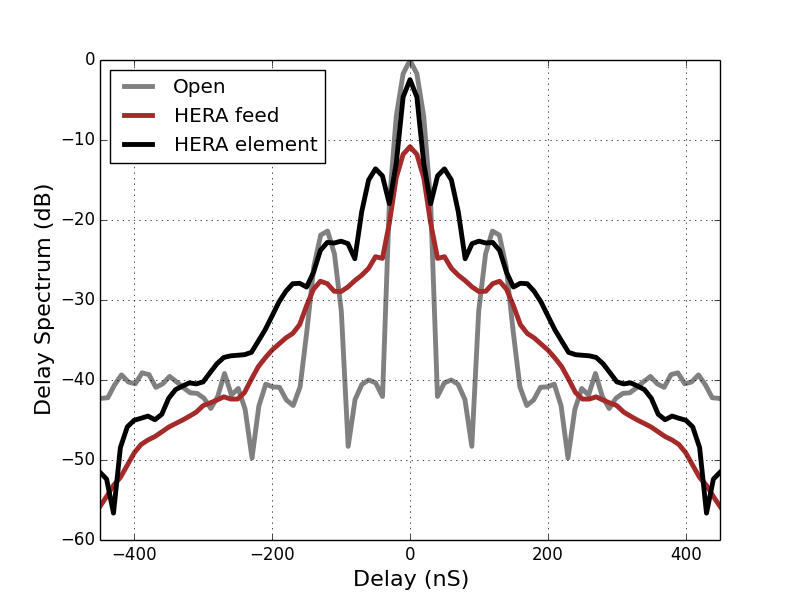
\includegraphics[angle=0, width=\linewidth]{GB_reflectometry_part3/plot/open_delay.png}
    \end{minipage}
    \caption{Left: Magnitude (blue) and phase (black) of the return loss measured when the open load is connected at the feed input of the cable. Ideally, for an open load, the electromagnetic wave traveling through the transmission cable undergoes a $100\%$ reflections and magnitude of the return loss is 0~dB. However, due to the resistive loss in the cable, the a small part of the signal is dissipated in the cable resulting a smaller return loss.  Right: Delay spectrum of the open load that shows the multiple reflections at the VNA input. The delay spectrum of the feed and the feed-dish assembly is also plotted for comparison.}
    \label{fig:open_RL}       
    \end{figure*}
    
    \subsection{Measurement bandwidth and window function}
    
    Estimation of the delay spectrum by taking the Fourier transform of the
    measured return loss is sensitive to the bandwidth of measurements. Since the
    measurements are done in the spectral domain over finite bandwidth, it is analogous
     to windowing the frequency domain data by a square
    window function. In the delay domain, the Fourier transform of this would result in
    multiple side lobes at higher delays. \textbf{Appropriate windowing of the
    measured data prior to taking the Fourier transform reduces
    the system response at higher delays by few orders of magnitude~\citep{nithya_et_al2013, Thyagarajan_et_al2016}.}
    figure \ref{fig:window} shows the delay spectrum estimated from the measured
    data using a square window as well as Blackman-Harris window. Even though windowing 
    results in about 50~$\%$ loss of spectral sensitivity, it may provide an additional 30~dB of headroom 
    for the foreground contaminations at higher delays. Loss of spectral sensitivity due to windowing could be compensated by longer integration
    time.     
    \begin{figure}
    \centering
    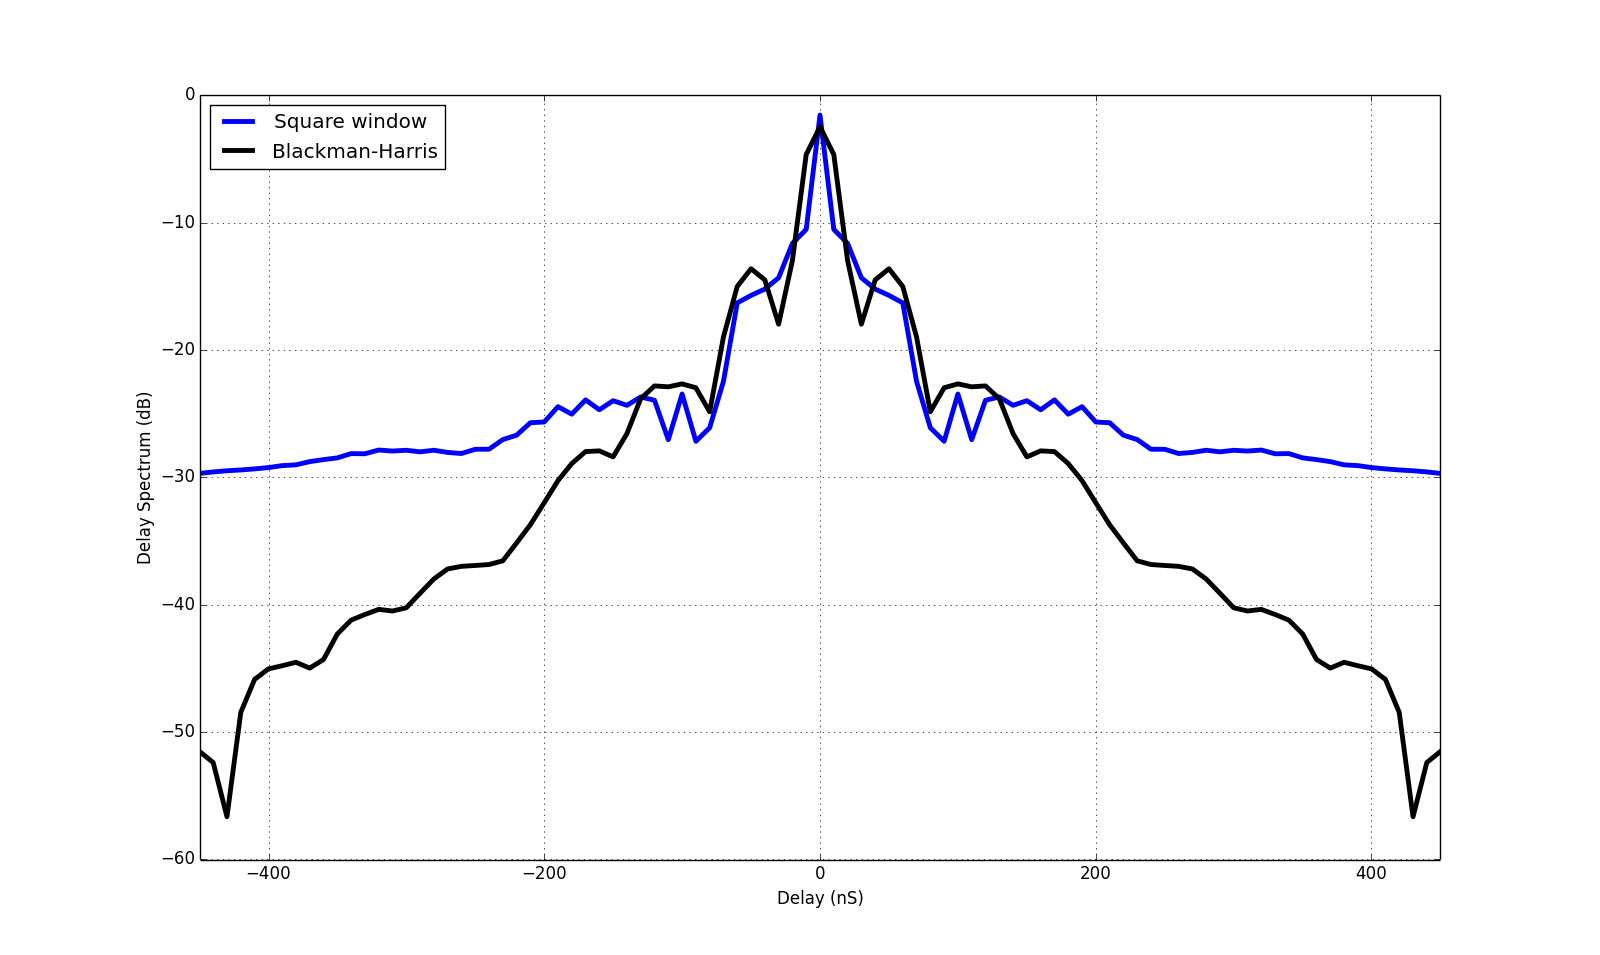
\includegraphics[width=\linewidth]{GB_reflectometry_part3/plot/ds_window.png}
    \caption{Effect of finite bandwidth on estimation of delay spectrum: Blue line shows the delay spectrum of the HERA element computed from the measured data which is band limited between 100 to 200~MHz. Black line shows the delay spectrum estimated from the same data set after multiplying the data by a Blackman Harris window. The delay spectrum of the windowed data set shows significant reduction in the instrument response at higher delays.}
    \label{fig:window}
    \end{figure} 
    
    %While measuring the return loss of the dish-feed assembly, the signal transmitted by the VNA is reflected first off the feed. This is represented by $\Gamma_{f}$ in equation \ref{eq:power_ratio}. This essentially represents a mismatched impedance between the feed and the 50 Ohm transmission line. In the delay domain, this appears at the zero delay bin. This response is identical whether or not the feed is suspended on the dish. We can, therefore, quantify this response by measuring the feed return loss while the feed is kept on the ground facing the sky. This results in a feed return loss including the surrounding cage structure but excluding the dish response. While a fraction, $\Gamma_{f}$, of the power is reflected off the feed, $1+\Gamma_{f}$ gets transmitted. In the receiving mode, upon initial incidence, $\Gamma_{f}$ of the voltage is reflected back into free space while $1+\Gamma_{f}$ enters the feed, and, in the delay domain, this appears at the zero delay bin. Using the return loss measurement of the feed $(\Gamma_{f})$ and the return loss measurement, $s_{11}$, of the dish, the feed assembly is corrected via equation \ref{eq:power_ratio} for the zero delay component, and the quantity of interest ${I_{rec}\over I_{sky}}$ is estimated. 
    %
    %
    %\begin{figure}[ht]
    %\centering
    %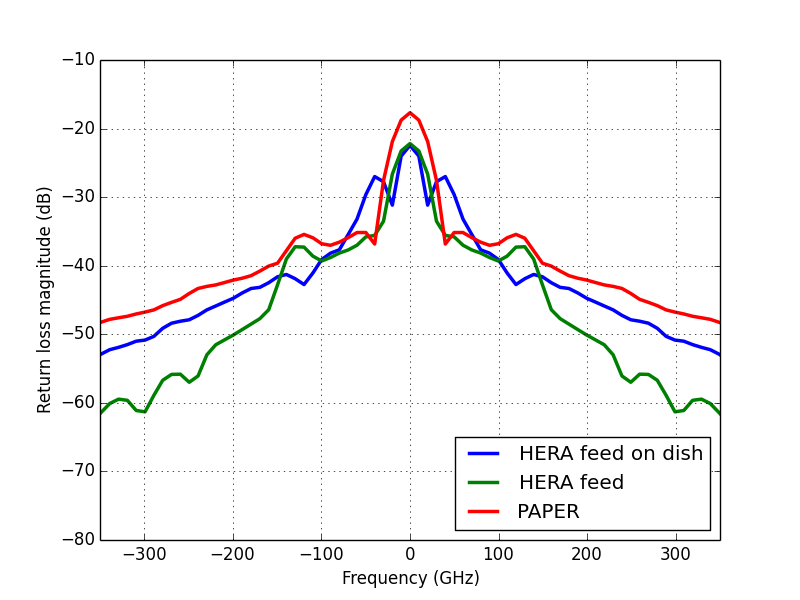
\includegraphics[width=\linewidth]{plots/delay_spectrum_100_200_BH.png}
    %\caption{Delay spectrum of the HERA element, the PAPER element, and the HERA feed estimated by taking the Fourier transform of the measured return loss of power at the feed output. The HERA feed design is driven by the PAPER element with an improved response at all delays. The feed, when suspended on the dish, results in a more complex return loss, and the corresponding delay response is shown in the figure.} %Delay units are incorrect!!!! Should be ns not GHz!!!!
    %\label{fig:delay_spectrum}
    %\end{figure}
    
  \subsection{Comparison with simulations}
  \begin{figure}{H}
  \centering
  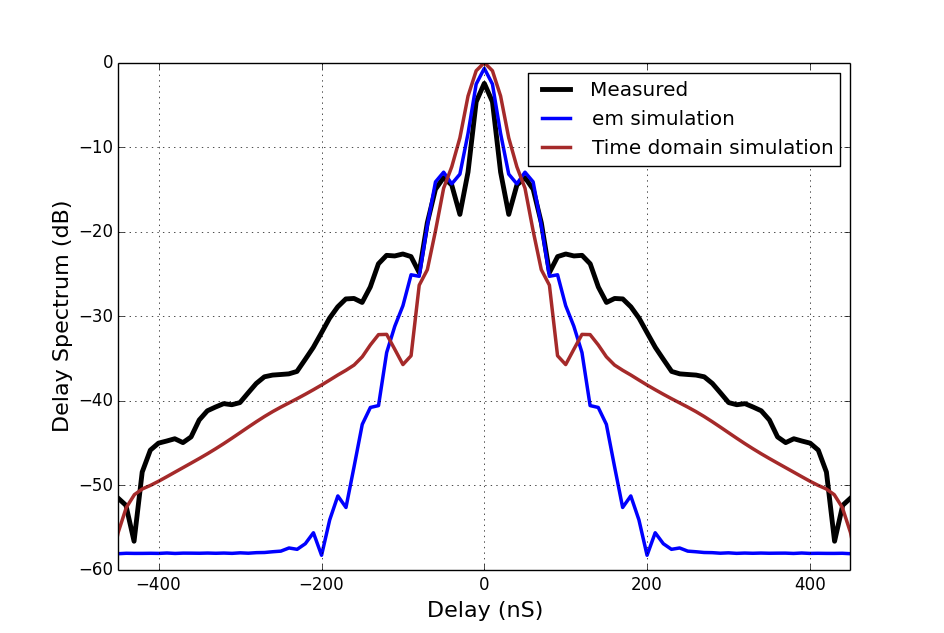
\includegraphics[width=\linewidth]{GB_reflectometry_part3/plot/simulation_comparison2.png}
  \caption{Delay spectrum of HERA element estimated from the reflectometry measurements by a vector network analyser compared to the delay spectrum estimated from the EM simulation using HFSS and time domain simulation using CST .}
   \label{fig:sim_em}
   \end{figure}
   
 \subsubsection{HFSS Electromagnetic simulation:}  
 Performance of the HERA feed and the HERA element has been simulated by
    using the EM solver "High Frequency Structural Simulator (HFSS)" using the finite
    element method.  The simulated and measured return loss of the feed, both
    magnitude and phase are shown in the upper panel of figure
    \ref{RL_mag_dish}. Bottom panel of figure \ref{RL_mag_dish} shows the measured return loss when
    feed is suspended at the focal plane of the parabolic dish which is at $4.5m$
    from the dish vertex. The measured return loss is much more complex than what
    is found from simulation. 
    While the simulated return loss of the feed structure shows
    two resonant peaks around 120 and 160~MHz, the feed resonance occur at
    slightly higher frequencies. Notable are the difference in the shape of the
    resonant peaks. While the simulated response shows very wide resonant peaks, as
    expected from these dipole structures, the measured return loss has
    a narrow peak at its low frequency resonance. The dominant term in the expression of  return loss of the HERA element in
    receiving mode (equation \ref{eq11}) is the zero delay term $(1+\Gamma_{f})$. Hence the feed return loss and especially the shape of the low frequency resonant peak dominates the overall shape of the delay spectrum in figure
    \ref{fig:sim_em}. 
 \textbf{The simulated return loss of the feed shows smooth variation across the band and wide resonant peaks resulting in a narrow delay spectrum.}
    
    
   \subsubsection{CST Time domain simulation:}  
    We also compare our measurements with the time domain simulation presented in ~\cite{Ewall-Wice_et_al2016} in figure \ref{fig:sim_em}. In this simulation, the transient electromagnetic response of the HERA element is determined as a function of time when it is subjected to a plane wavefront. The commercial numerical simulation software Microwave Studio, developed by Computer Simulation Technology is used for the simulation. The simulation assumed a constant 125~$\Omega$ impedance at the dipole terminal. Therefore, delay spectrum estimated from this simulation only has the effects of chromaticity introduced due to the structural reflections. In practice, dipole impedance is function of frequency that results in variation of return loss with frequency. This results in deviation between the simulated delay response and the delay spectrum estimate of our measurements. \\
     \subsubsection{Foreground simulation:}  
    We also compare our measurement with the foreground simulation of~\citep{Thyagarajan_et_al2016} as shown by the shaded regions in the first panel of figure \ref{ds_full_sub_band}. The shaded region of each panel shows the EoR to
    foreground power ratio required for detection of 21~cm power spectrum at those
    individual delays. This ratio is computed by
    using the HFSS simulation of chromatic antenna beam and the sky models. Diffused foreground sky model is
    incorporated from~\citep{deolivieracosta_et_al2008} whereas the point source
    contribution is estimated by combining the NRAO VLA Sky Survey (NVSS) at
    1.42~GHz~\citep{Condon_1998}, Sydney University Molonglo sky Survey (SUMSS)
    ~\citep{Bock_et_al_1999, Mauch_et_al_2003} at 843~MHz. The EoR signal
    is simulated by using 21cmFAST \citep{Messinger_et_al2011}. The model
    parameters used for the EoR signal simulation
    are : Virial temperature of minimum mass of dark matter halos that host
    ionizing sources, $T_{vir}^{min} = 2\times10^4$~K, Ionising efficiency $\eta = 20\%$,
    mean free path of UV photons $R_{mfp} = 15$~Mpc For these model parameter
    values, the redshift of $50\%$ reionization is predicted to be at $z = 8.5$ at
    150MHz.  
    The EoR to foreground power ratio shows that for a given
    delay mode, the estimate of a lower $k_{\parallel}$ mode requires a higher
    attenuation compared to a higher $k_{\parallel}$ mode. 
    \textbf{This simulation provides a baseline for the system performance evaluation with a conservative strategy of pure foreground avoidance without any foreground mitigation strategy. The measurements differ from the simulation in one aspect. Simulation includes the frequency dependent antenna gain which does not include the return loss of of power at the antenna terminal due to frequency dependent antenna impedance. This effect is included in the measurements.
  If included in the model, these limits would provide more conservative estimates of the required instrument response which will be even harder to achieve.}
     % Hence, the shaded region shows the most      
   %  stringent limits of EoR to foreground power ratio and sets the upper most limit of the required system performance under    
     %the assumption of non-chromatic return loss. 
     
    \subsubsection{Delay spectrum of sub bands}
    \label{sub-band}
    In the HERA analysis, the 21~cm power spectrum
    is estimated by discretizing the observed data along the line of sight distance i.e
    in frequency or redshift and in the plane of the sky
    $k$~\citep{liu_et_al2014a}. At particular redshift, the bandwidth of
    observation is so chosen that over the corresponding $\Delta z$, the 21~cm
    signal does not significantly evolve. Typically, the the 21~cm brightness
    temperature fluctuation evolves over redshift scale $\Delta
    z>0.5$~\citep{loeb_zaldarriaga2004},~\citep{lidz_et_al2008}. Therefore, the delay
    spectrum is estimated over smaller bandwidths.
    
    We estimate the instrument
    delay spectrum over various sub bands between 100 to 200~MHz as shown in figure
    \ref{ds_full_sub_band}. Each panel of figure \ref{ds_full_sub_band} shows the
    delay spectrum estimated from the return loss measurement of the HERA element
    between 100-200, 100-140, 130-170, 160 to 200~MHz respectively. Each panel also
    compares the delay spectrum estimate obtained EM simulation of~\cite{deBoer_2016} at various subband. Subband delay spectra are wider compared to full
    band delay spectrum.  The shape of the resonant peaks determines the roll off rate
    of the delay spectrum at all frequency ranges. At higher
    frequency, our measurement closely follows the EM simulations except around
    80-120~ns where the cable reflection between the antenna and the backend manifests
    itself. 
    
    The shaded regions represent the EoR to Foreground power ratio simulated across the entire band.
    The HFSS simulation of chromatic antenna beam varies smoothly across frequency resulting in no significant changes in this simulation at various sub bands.  
     HERA system performance conforms directly to the limits as posed by simulations, at frequencies $>$160~MHz. With the measured system response including the multiple reflections, the instrument would be able to probe the spatial modes of interest $k_{\parallel}>0.2 h$~Mpc$^{-1}$ with very little foreground bleeding around $k_{\parallel} \approx 0.2 h$ Mpc$^{-1}$.
      At other frequencies, it is possible to do a successful measurement by weighting down the
      foreground contribution in the measured data. This is discussed in the following section.
    \begin{figure*}[ht]
    \begin{minipage}[b]{0.5\linewidth}
    \centering
    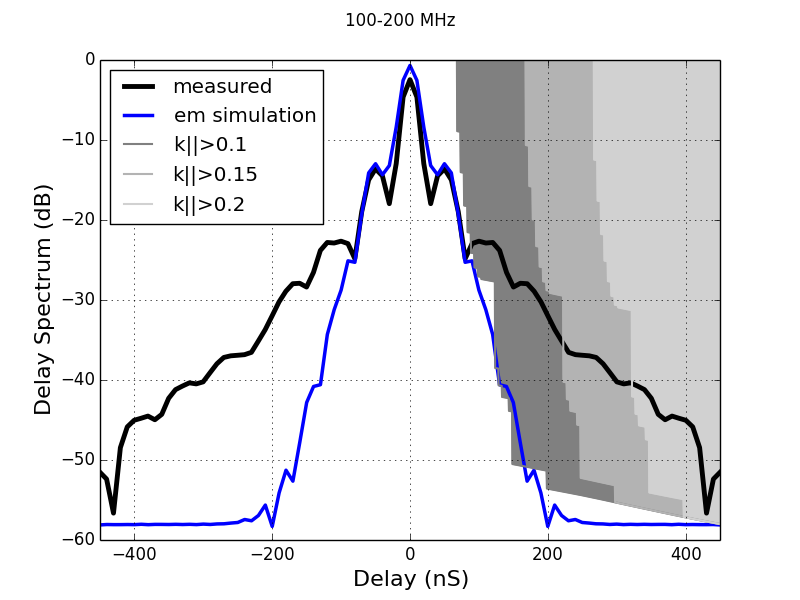
\includegraphics[angle=0, width=\linewidth]{GB_reflectometry_part3/plot/100_200.png}
    \end{minipage}
    \hspace{0.1cm}
    \begin{minipage}[b]{0.5\linewidth}
    \centering
    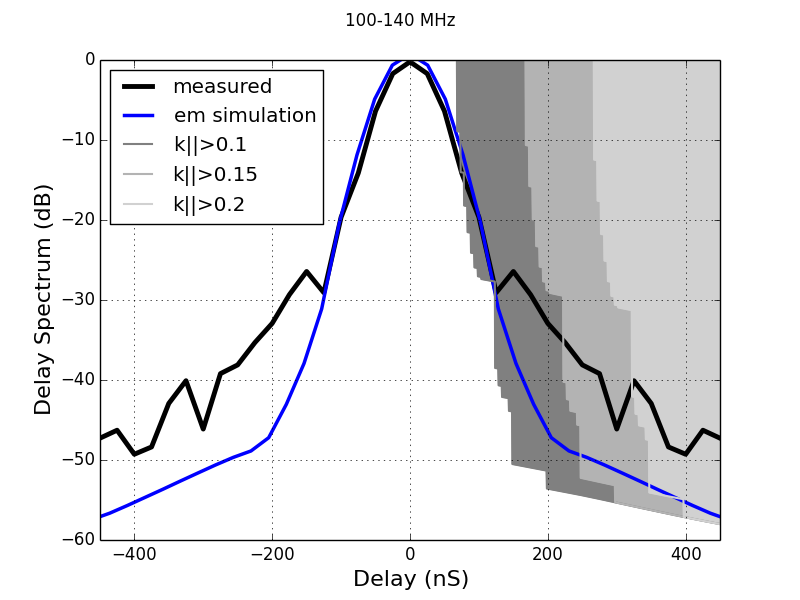
\includegraphics[angle=0, width=\linewidth]{GB_reflectometry_part3/plot/100_140.png}
    \end{minipage}
    \vspace{0.1cm}
    \begin{minipage}[b]{0.5\linewidth}
    \centering
    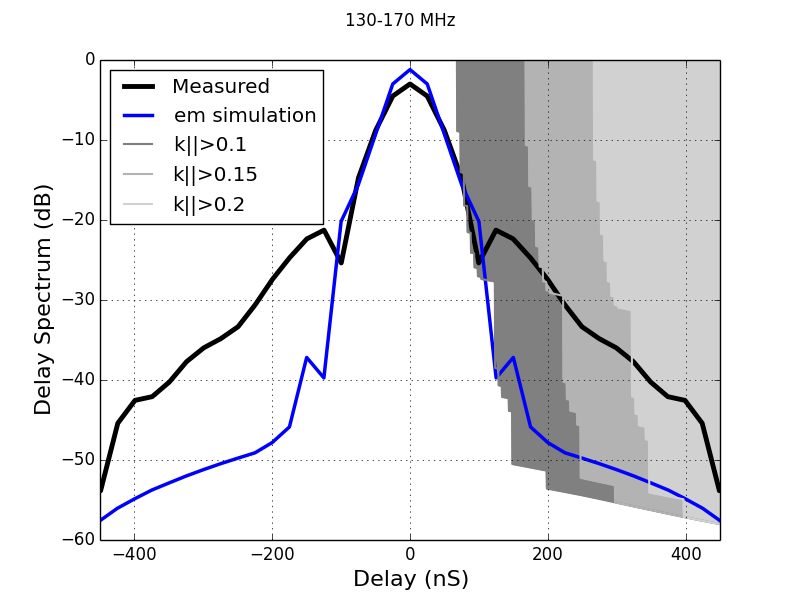
\includegraphics[angle=0, width=\linewidth]{GB_reflectometry_part3/plot/130_170.png}
    \end{minipage}
    \hspace{0.1cm}
    \begin{minipage}[b]{0.5\linewidth}
    \centering
    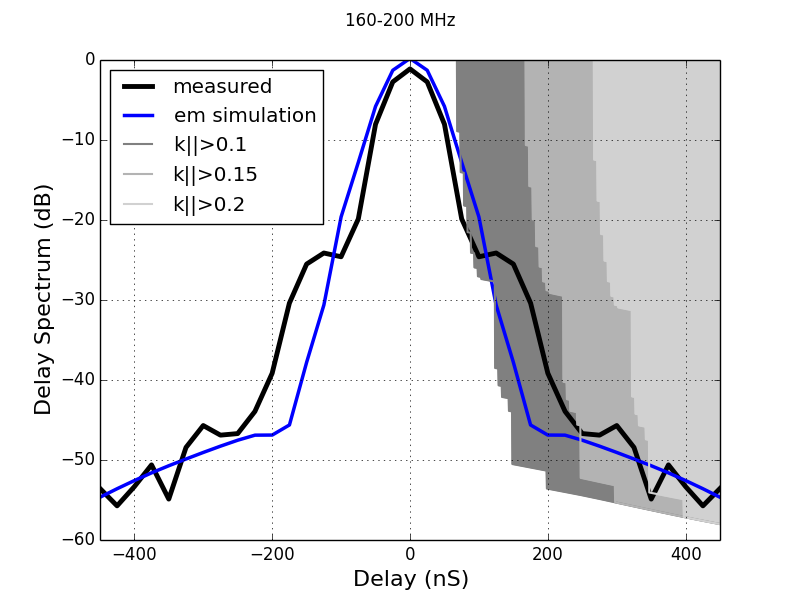
\includegraphics[angle=0, width=\linewidth]{GB_reflectometry_part3/plot/160_200.png}
    \end{minipage}
    \caption{Delay response of the instrument estimated from the measurements of the complex return loss of the HERA element and the feed (black). The blue curve shows the same estimated from the EM simulation of the feed and the HERA element. The shaded gray regions shows the ratio of the EoR to foreground power required to detect the EoR power spectrum at a given delay. At a given delay, detection of EoR power spectrum at smaller $k_{\parallel}$ mode requires higher attenuation of the foreground power. This is shown by three different shaded region. The instrument delay response estimated over the full band is dominated by the sharpest feature present in the observation band. At $120~MHz$, the feed impedance is best matched to the 50~$\Omega$ reference impedance providing a very low value of return loss. This feature, when Fourier transformed to delay domain results in a wide response.  At higher frequencies , the measured return loss varies smoothly with frequency resulting in narrow delay response of the instrument. }   
    \label{ds_full_sub_band}
    \end{figure*}
 The HERA analysis pipeline for power spectrum estimation exploits the inverse covariance weighting to reduce the foreground contribution to the measured visibility data. In the light of this analysis technique we further investigate the limits of EoR to foreground power ratio from what is established by conservative estimates of \cite{Thyagarajan_et_al2016}. In the following section we briefly describe the power spectrum estimation technique used in HERA analysis and inverse covariance weighting. We evaluate the instrument delay response in the context of covariance weighting.

   % \section{\textbf{Power spectrum estimation}}  
   \section{\textbf{Revised delay spectrum specification using inverse covariance weighting}}    
    The results we presented in the previous section focused on the delay-domain performance of
the antenna, where it convolves the foreground signal and must fall beneath the amplitude of the 
21cm EoR signal to avoid a systematic bias.  We used a windowed delay tranformation to make these comparisons.
This simple analysis lends itself to being easily interpretable, but it omits the 
suppression of foreground systematics that are a feature of more sophisticated power spectrum estimation techniques.
In this section, we explore how we might re-evaluate our specification for the delay-domain performance of
the HERA antenna in light of these techniques.

    HERA power spectrum estimation is done using the optimal quadratic estimator
    (OQE) formalism that has been outlined in extensive detail in  ~\cite{liu_et_al2010}, ~\cite{dillon_et_al2013a}, ~\cite{liu_et_al2014a}, ~\cite{liu_et_al2014b}, ~\cite{trott_et_al2012}, ~\cite{Ali_et_al2015}. We briefly  describe the major steps of OQE formalism here and evaluate the prototype HERA element response in the light of this analysis method.
    
The 21~cm power spectrum $P_{21}(k_\perp,k_\parallel)$ is related to the temperature field as, 
    \begin{equation}
    \langle  \tilde T_{b}(\bold k) \tilde T_{b}^{*}(\bold k^{'}) \rangle = (2\pi)^{3} \delta (\bold k - \bold k^{'})P_{21}(k_\perp,k_\parallel)
    \label{eq14}
    \end{equation}
    
    where $\langle  \tilde T_{b}(\bold k) \tilde T_{b}^{*}(\bold k^{'}) \rangle $ is the correlation function of the three dimensional spatial Fourier transform of the sky brightness temperature distribution $ \tilde T_{b}(\bold k)$, and $\delta$ is the Dirac delta function. %While both $P_{21}(k_\perp,k_\parallel)$ and $\tilde T_{b}({\bold k})$ are continuous, the power spectrum estimate is discrete. Observation frequency and bandwidth are so chosen that the power spectrum is approximated as a constant and a piecewise discrete function of $\bold k$  which correspond to a thin shell in $\bold k$ space assuming isotropy perpendicular to the line of sight. 
 %This corresponds to the $k_{\perp}$, $k_{\parallel}$  values $a <k_{\perp} < a+1$, $b <k_{\parallel} < b+1$ where the indices a, b can assume M, N different values.  
 We estimate the power spectrum $P(k)$ integrated over a range of $k_\parallel, k_\perp$.  We call this 
the bandpower $\hat p_{\alpha}$, where $\alpha$ represents a range of $k_{\parallel}, k_{\perp}$. Let us take
$\bold x$ to be a vector of visibilities measured at range of frequencies.  We can estimate unnormalized
band powers $\hat q_\alpha$ according to the equation
    \begin{equation}
    \hat q_{\alpha} = \bold x^{T} E^{\alpha} \bold x, % - b_{\alpha}
    \label{eq15}
    \end{equation}
 %   where $b_{\alpha}$ is additive noise bias  to the power spectrum estimate. In practice, $b_{\alpha}$ can be eliminated from the estimate by cross correlating two visibility data sets with different noise terms. 
 where $E^{\alpha}$ is a symmetric matrix operation denoting the Fourier transform of the data, binning, and foreground reduction. Various binning and foreground reduction techniques result in different forms of $E^{\alpha}$ resulting in estimates of $\hat p_{\alpha}$ with different statistics. A possible choice of $E^{\alpha}$ is
    \begin{equation}
    E^{\alpha} =  {1 \over 2} C^{-1} Q_{\alpha} C^{-1}
    \label{eq16}
    \end{equation} 
    
    where $C = \langle \bold x \bold x^{t} \rangle$ is the covariance matrix of the data vector $\bold x$. $Q_{\alpha}$ is a matrix operator that Fourier transforms the visibilities along the frequency axis and maps them into the $\bold k$ space. Finally, the normalized estimate of the power spectrum could be written as,  
    \begin{equation}
    \hat p_{\alpha} = M \hat q_{\alpha} 
    \label{eq17}
    \end{equation} 
    where $M$ is the normalization matrix.
 The true power spectrum $p_{\alpha}$ is related to $\hat p_{\alpha}$  by the window function matrix $W$, 
    \begin{equation}
    \hat p_{\alpha} = W p_{\alpha}
    \label{eq18}
    \end{equation} 
    
   % Hence, the estimated power spectrum $\hat p_{\alpha}$ for a given $\bold k $ values would have contribution for the nearby $\bold k$ values weighted by the window function.% The wider the window function, the larger would be the contribution of the adjacent modes to the discrete power spectrum estimate. 
%In general, $W$ is a non-diagonal matrix. For a given choice of normalization matrix M, the window function W will be, 
    
   % \begin{equation}
    % W = MF
     %\label{eq19}
    %\end{equation} 
    
   % where , 
    %\begin{equation}
     %F_{\alpha\beta} = \frac {1} { 2} [C^{-1}Q_{\alpha}C^{-1}Q_{\beta}]^{T}
     %\label{eq20}
    %\end{equation} 
     %is the Fisher matrix of the measured data. The choice of normalization matrix $M$ is critically important for the analysis. If $M \propto F^{-1}$, $W\propto I$ resulting in $\hat p_{\alpha} = p_{\alpha}$ i.e, estimated value of the power spectrum equals to the true power spectrum.\\
     %The errors on the power spectrum estimate is given by the covariance of the band power which could be computed from the measured data as,  
    %\begin{eqnarray}
     %C_{\alpha, \beta} %& = & \langle \hat p_{\alpha} \hat p_{\beta}^{T} \rangle - \langle \hat p_{\alpha} \rangle \langle \hat p_{\beta}^{T} \rangle \nonumber\\
     	%	& = & MFM^{T}
    %\label{eq21}
     %\end{eqnarray} 
     
     %For a choice of $M \propto F^{-1}$, the covariance in the estimated band power is as large as $M$ resulting in highest error in estimation. Hence, the choice of the normalization matrix $M$ is critical in the analysis process since its precise form determines the vertical error bars in the estimate of power spectrum. 
    
   % \subsection{Inverse covariance weighting: revised delay spectrum limit}
  The critical step in the power spectrum estimation formalism is the weighting of the data by the inverse of its covariance. This can result in orders-of-magnitude reduction in the foreground power relative to the EoR signal because foregrounds tend to be concentrated into a small number of eigenmodes. 

To derive a delay-spectrum specification for an antenna using the inverse covariance weighting, we begin
with the
   simulations of \cite{Thyagarajan_et_al2016} and use OQE formalism to estimate the amplitude of the power spectrum
from a simulated data vector $\bold x$ 
    which contains contributions from the EoR, the foreground, and
   the instrument noise. The computed power spectra with and without covariance weighting are shown in figure \ref{fig:cov_weight}, where the strong dependence of the foreground amplitude on the weighting of the data can be clearly seen. The orange curve indicates the power spectrum computed from the EoR model averaged over three different baseline orientations for adjacent HERA elements.  The blue curve indicates the power spectrum of the observed sky signal including both foreground and the EoR using the windowed delay transform analysis. Here, the contribution from the bright foregrounds dominate the lower delay modes, making separation of the EoR from the foreground impossible up to delays $\approx 300$ ~ns. 
   % The matrix $E^{\alpha}$ represents a weighting of the data vector $\bold x$ by inverse of its covariance.
The covariance weighted power spectrum is illustrated by the purple curve in the plot. 
   Weighting by the covariance matrix estimated from the simulated data dramatically reduces the foreground power relative to the EoR signal at low delays, opening up the possibility of estimating the EoR power spectrum at those delays. 

When using simple delay-transform power spectrum estimation, the chromaticism of the antenna convolves
the foreground signal in delay domain.  As described in \ref{Thyagarajan_et_al2016}, this 
enables us to set a specification
for our antenna reflectometry as a function of delay, as illustrated by the grey shaded regions in
Figure \ref{fig:sim_fg_revised}.  This relationship is not as simple when using
optimal quadratic power-spectrum estimation.  For example, a direction-independent bandpass shape 
that multiplies the foreground signal falls into a single eigenmode that can be downweighted essentially to zero.
This makes the interpretation of the output power spectrum as a reflectometry constraint problematic.  Without
knowing in detail the direction dependence of the antenna chromaticism, we cannot know how many eigenmodes
will be occupied by the systematics arising from the foreground-dish interaction. 

To be relatively conservative, we simply use the inverse covariance weighted power spectrum from simulations that
do not include antenna chromaticism as an effective input foreground amplitude and repeat the translation to
a reflectometry specification as before.  The result is illustrated by the colored shaded regions
in Figure \ref{fig:sim_fg_revised}.  This approach ignores the ability of OQE to identify and invert
instrumental covariances, making it a relatively conservative standard.  On the other hand, should the number
of direction-dependent spectral eigenmodes of the dish become large, this approach could potentially underestimate
the impact of dish chromaticism.  Therefore, we present it as a demonstration that our reflectometry specifications
could be substantially less stringent for HERA's OQE pipeline, but suggest not over-interpreting the exact 
level of the implied specification without a detailed analysis of the direction dependence of the reflectometry
results.

    %Strongsystematics that appear in the covariance of $\bold x$ will appear as eigen modes
    %of $C$, which will be downweighted in $C^{-1}$ by the square of their corresponding
    %eigenvalue.
    \begin{figure}
    \centering
    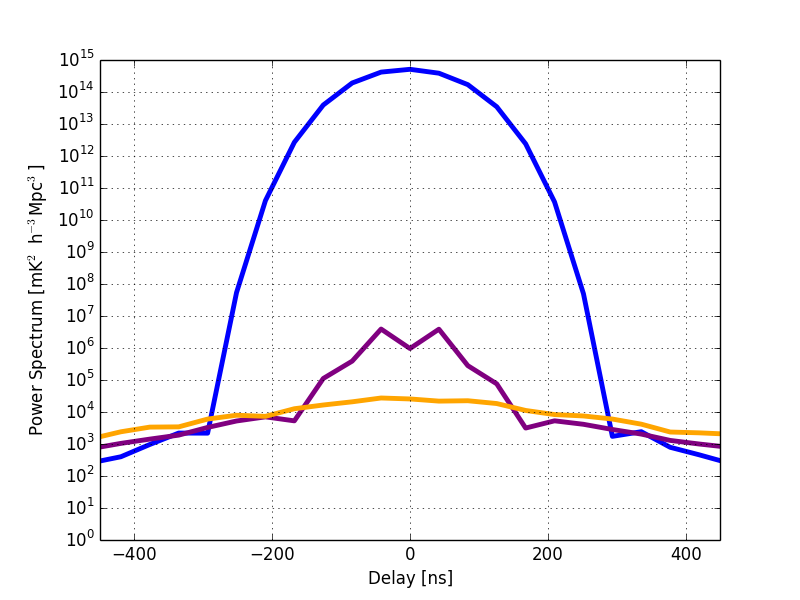
\includegraphics[width=\linewidth]{GB_reflectometry_part3/plot/figure_cov_weight.png}
    \caption{The HERA feed consists of a pair of crossed-dipoles over 1.72 m diameter backplane made of wire mesh. The backplane is surrounded by 0.36 m wide wire mesh around the edge resulting in encasing the crossed-dipoles in a cylindrical cage.}
    \label{fig:cov_weight}
    \end{figure}
      %The chromaticity of HERA element introduces a (potentially direction dependent) frequency
     %covariance in our data. As a result, the
     %covariance convolves bright foregrounds in $\bold k$-space,
     %foreground spills into $\bold k$ modes outside the maximum geometric
     %delay where they contaminate measurements of the EoR power spectrum.
     %Weighting the measured visibility by the inverse of its
    %covariance results in orders-of-magnitude reduction in foreground power relative to
    %the EoR signal.
    %In this sense, using optimal quadratic estimators can dramatically 
    %reduce our reliance on smooth instrumental responses, with a corresponding reduction
    %in the stringency of instrument performance specification.
    
     %We again compute the required attenuation of foreground power relative to the EoR signal at every delay and compare it with the delay response of the instrument. \textbf{This ratio now has higher values at each delay in comparison with the conservative estimate provided by \cite{Thyagarajan_et_al2016} as shown in fig: \ref{fig:sim_fg_revised}. }
     %Combining the inverse covariance weighting formalism with the
    %foreground simulation of \cite{Thyagarajan_et_al2016}, we derive a new specification on
    %foreground attenuation with respect to the EoR signal required for
    %power spectrum estimation. The foreground model of
    %\cite{Thyagarajan_et_al2016} as described in section \ref{sub-band} is adopted here. %We use
   % the reflectometry measurements, corrected for the antenna response in the
    %receiving mode (eq \ref{eq11}) to compute the visibilities for the given model of the
    %foreground, the EoR and the system noise. 
     %\textbf{Our measurement includes chromaticity of the beam as well as antenna impedance as a function of frequency i.e, the effect 
     %of return loss of power at the antenna terminal. Angular response of the antenna beam 
     %can also be a function of frequency and introduce additional modes of fluctuations. This is included in the conservative estimates of \cite{Thyagarajan_et_al2015}. Our
     %measured response is beam integrated and does not take into account this angle dependency.}
     %These visibilities formed the complex
    %data vector $\bold x$. We compute the covariance matrix $C$ from the simulated
    %data. It is hard to know the
    %covariance of systematics in $\bold x$ prior to estimating them from the data. In
    %practice, the total covariance matrix $C$ is often estimated from the measured
    %visibilities themselves~\citep{Ali_et_al2015}. 
    %$\bold x$ is then multiplied by the inverse of the covariance matrix.
    %This step essentially weighs down the foreground contribution to the measured
    %data. Once Fourier transformed, the delay spectrum of the simulated data is
    %constituted by linear super position of the delay spectrum of the foreground,
    %and the EoR signal.
      
    
    \begin{figure*}
    \centering
    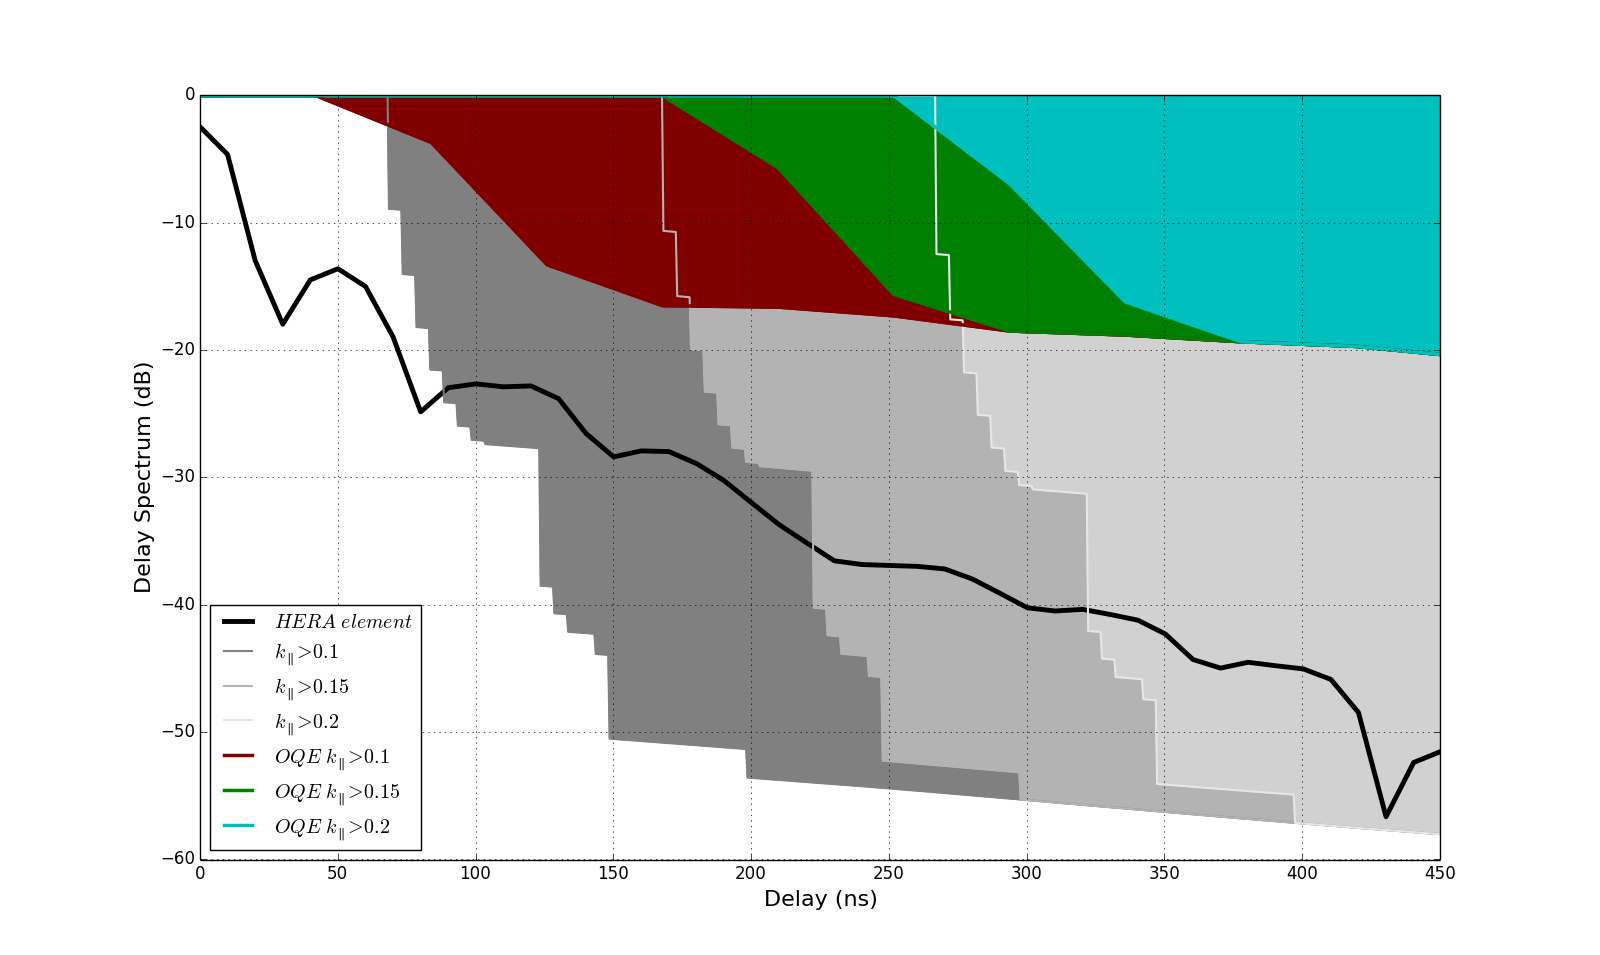
\includegraphics[width=\linewidth]{GB_reflectometry_part3/plot/HERA_ds_fg_sim_revised.png}
    \caption{Delay spectrum of HERA element estimated from the reflectometry measurements by a vector network analyzer. The colored region shows the revised EoR to foreground power ratio in comparison to our measurements and the conservative estimates presented in \cite{Thyagarajan_et_al2016}. Once again it is shown that for a given delay, power spectrum estimate for a small $k_{\parallel}$ value requires higher attenuation of foreground power with respect to EoR. However, due to inverse covariance weighting of the visibility, the foreground contribution at each delay is reduced relaxing the limits on the required attenuation by about $30~dB$ at each delay.}
    \label{fig:sim_fg_revised}
    \end{figure*}
   \textbf{ This demonstrates that the performance of the HERA element including it intrinsic chromaticity and chromaticity generated due to multiple reflections in the system. The prototype HERA element delay response, in conjunction with the inverse covariance method of foreground suppression, indicates that the HERA can make a successful power spectrum measurement for the spatial modes as low as $k_{\parallel} >0.1 h$ Mpc$^{-1}$.} 
    %Covariance matrix $C$ is computed from the simulated visibility data. Next, the data vector $\bold $ that consists of the complex simulated visibilities, is weighted by the computed covariance of the data. 
    %instrument delay response for power spectrum measurements. With inverse covariance weighting a %foreground suppression of about 30dB could be achieved that results in room for substantial %performance degradation and yet a successful measurement of 21~cm power spectrum. Our %measurements, evaluated in the light of these limits shows that the HERA is not limited by either its %systematics. With only delay spectrum technique, it is capable of detecting the EoR power spectrum %for the $k_{\parallel}$ modes as low as $k_{\parallel}>=0.2$. If combined with the inverse covariance %weighting formalism of foreground suppression, the instrument performs well below the limits of %foreground suppression. We briefly describe the inverse covariance weighting formalism below.
    %\subsection{Inverse covariance weighting}
    %The 21 cm delay spectrum estimate and thus the 21~cm power spectrum, consists of three main components, the foreground power spectrum $\hat p_{FG}$, the EoR power spectrum $\hat p_{EoR}$and the noise power spectrum of the instrument.
    %\begin{equation}
    %\hat p =  \hat p_{FG} + \hat p_{EoR}+ \hat p_{noise}
    %\end{equation}
    %In the inverse-variance weighting, two or more random variables are aggregated to minimize the variance of the weighted average. Hence, weighting the estimated delay spectrum with the inverse variance of the foreground reduces the foreground contaminations in the measurements. 
    %would  for power spectrum measurements, especially at smaller spatial scales of fluctuation i.e lower values of $k_{\parallel}$.
    \section{\textbf{Conclusion}}
     \textbf{The interplay between the extremely bright sky signal and the system response
    has remained somewhat undetermined for the first generation 21cm experiments such
    as MWA, LOFAR, PAPER. With the theory of redshifted 21cm experiments very
    well evolved, it is now absolutely necessary to quantify the instrumental limits
    of these measurements in order to produce accurate power spectrum estimates.}
    
    
    In this paper, we studied the performance of a prototype HERA element in both frequency
    as well as delay domain. \textbf{In this paper, we have introduced a mathematical formalism that explicitly
    relate the delay response of the HERA element to EoR to foreground power ratio.}
    The effects of multiple reflections  in a HERA
    element is investigated in detail and their effects on the measured
    visibility as well as delay spectrum is estimated.  The delay-domain
    performance of the HERA dish is central to HERA's function as a power spectrum
    instrument. 
    
    Reflectometry measurements characterized HERA's performance in this
    domain and, as equation \ref{eq10} shows, these measurements must be adjusted
    for a difference in transmission/reception at the first feed encounter in
    order to be interpreted as the delay response of a feed relative to an incident
    plane wave from the sky.  It is also shown that the choice of windowing
    function is critical for accurately measuring the antenna delay response at
    higher delays, where sidelobes from much higher amplitude responses at small
    delays can easily dominate. The Blackman-Harris window is found to be generally
    adequate while square windowing functions are not.  Given the critical nature
    of the windowing function, it is recommended that all reflectometry
    measurements be performed in the frequency domain, so that the data could be
    Fourier transformed with the appropriate window.  The delay spectrum estimates
    are then compared with the electromagnetic as well as time domain simulation of
    the HERA element~\citep{ddboer_et_al2016, Ewall-Wice_et_al2016}. The
    same is then compared with the estimates derived from the foreground simulation
    of~\cite{Thyagarajan_et_al2016}. The performance is also evaluated in the light
    of HERA power spectrum estimation technique using inverse covariance weighting
    formalism.  Taken all together, we conclude that the HERA antenna element,
    with a PAPER-style crossed dipole feed and cylindrical cage, satisfies the criteria necessary to meet its science
    goal. \\
    
    {\bf Acknowledgements:}  
This work was supported by the U.S. National Science Foundation (NSF) through awards AST-1440343 and AST-1410719.
ARP acknowledges support from NSF CAREER award 13

52519.
AL acknowledges support for this work by NASA through Hubble Fellowship grant \#HST-HF2-51363.001-A awarded by the Space Telescope Science Institute, which is operated by the Association of Universities for Research in Astronomy, Inc., for NASA, under contract NAS5-26555.
This research was completed as part of the University of California Cosmic Dawn Initiative. AL, ARP, and SRF acknowledge support from the University of California Office of the President Multicampus Research Programs and Initiatives through award MR-15-328388

    %\bibliography{biblio}{}
    \bibliographystyle{apj}
    \bibliography{Reference}{}
    
    \end{document}
    
 
